% main.tex -- owner: merging task.  Section owners: request changes through NOTES.md.
% Build: pdflatex main; bibtex main; pdflatex main; pdflatex main
\PassOptionsToPackage{expansion=false}{microtype}
\documentclass[a4paper,UKenglish,cleveref,autoref,thm-restate]{lipics-v2021}

\usepackage{booktabs}
\usepackage{multirow}
\usepackage{xcolor}
\usepackage{xurl}
\usepackage{tikz}
\usetikzlibrary{positioning,decorations.pathreplacing,arrows.meta}
\hideLIPIcs

% Macros from KATKA
\newcommand{\TODO}[1]{\textcolor{red}{[TODO: #1]}}
% Macros from More RLBWT Tricks
\newcommand{\intv}{I}
\newcommand{\Rref}{R}
\newcommand{\pend}[1]{\textcolor{red}{#1}}
\newcommand{\succp}{\mathit{succ}}
\newcommand{\Pa}{\Pi}

\title{Three Examples of MEM-Finding}
\titlerunning{Three Examples of MEM-Finding}

\author{Travis Gagie}{CeBiB -- Center for Biotechnology and Bioengineering, Chile}{travis.gagie@gmail.com}{https://orcid.org/0000-0003-3689-327X}{}
\author{Gonzalo Navarro}{Department of Computer Science, University of Chile, Santiago, Chile \and CeBiB -- Center for Biotechnology and Bioengineering, Chile}{gnavarro@dcc.uchile.cl}{https://orcid.org/0000-0002-2286-741X}{}

\authorrunning{T. Gagie and G. Navarro}
\Copyright{Travis Gagie and Gonzalo Navarro}

\ccsdesc[500]{Theory of computation~Data structures design and analysis}
\ccsdesc[500]{Theory of computation~Pattern matching}
\ccsdesc[300]{Applied computing~Bioinformatics}
\keywords{Maximal exact matches, Boyer--Moore--Li, run-length compressed Burrows--Wheeler transform, RLCSA, tag arrays, taxonomic classification, two-level indexing, syncmers, pangenomics}

\supplement{All code and scripts: \url{https://github.com/TravisGagie/MEM-finding} (Sections~\ref{sec:zymo} and~\ref{sec:silva} in \texttt{katka/}, Section~\ref{sec:chr19} in \texttt{chr19/}).}

\acknowledgements{Many thanks to Ben Langmead for recommending classification with MEMs, and for asking, several years ago, whether BWT-based indexes could get the kind of sequential-access speed that $k$-mer indexes built on compacted de Bruijn graphs get once they reach a unitig; and to Omar Ahmed, Victor Alfaro and Christina Boucher.  The first author thanks Dr.\ Curtis Marcoux for leading the team that treated him for the past two years, Dr.\ Amy Trottier for convincing him that bioinformatics is actually useful, and the staff of the 4th and 8th floors of the Victoria General Hospital in Halifax.  The ideas in this paper are the authors'; the code, the experiments and the text were developed by Claude Opus 5.5, an AI model by Anthropic, under the authors' direction.}

\relatedversion{}

\EventEditors{John Q. Open and Joan R. Access}
\EventNoEds{2}
\EventLongTitle{42nd Conference on Very Important Topics (CVIT 2016)}
\EventShortTitle{CVIT 2016}
\EventAcronym{CVIT}
\EventYear{2016}
\EventDate{December 24--27, 2016}
\EventLocation{Little Whinging, United Kingdom}
\EventLogo{}
\SeriesVolume{42}
\ArticleNo{23}

\begin{document}
\maketitle

\begin{abstract}
Finding maximal exact matches (MEMs) with indexes based on the run-length compressed Burrows--Wheeler transform is a common core of read classification and pangenome search, but where the time goes depends on the data.
We describe three experiments, each with a different bottleneck and a different structure that removes it.
Most of these structures are known or easy combinations of known ones; what is new is mainly a comparison of credit schemes, a bound on the runs of tag arrays, and an encoding of a parse into blocks that lets two-level indexing cross long matches faster.
On long, noisy nanopore reads from whole genomes, the bottleneck is \emph{finding} the right matches: with homopolymer compression, a low-complexity filter, and each read's longest MEMs, found in one pass of Boyer--Moore--Li (BML) with an adaptive threshold and KeBaB's $k$-mer filter searched longest first, we assign 99.6\% of the reads to their species with no length threshold.
On short 16S rRNA reads classified to genera with SILVA, many MEMs occur in several genera and the bottleneck is \emph{answering} each MEM: credit proportional to the number of occurrences in each taxon is the most accurate split, by 1.0 to 6.8 percentage points, and a complete, run-length compressed tag array counts the occurrences in time proportional to the number of tag runs in the MEM's BWT interval, without locating any occurrence.
We bound the number of tag runs, and show that tags constant on $d$ segments of the text have a macro scheme with at most $r + 2d$ phrases.
Our index takes 1.44\,GB and classifies a read in 66\,$\mu$s at 93.8\% accuracy; on the same reads and server, it is 14 times smaller than Cliffy's undigested index, and 4.4 times faster and 8 points more accurate than Cliffy's LCA query on it.
On whole human chromosome~19 haplotypes against collections of 16 to 64 others, the bottleneck is \emph{crossing} long matches: two-level indexing with a closed-syncmer parse, encoded in blocks of phrases that are each the lexicographically smallest successor of the one before, crosses a whole block in one step and finds the MEMs 28 to 49 times faster than plain backward search, 6.4 to 11.2 times faster than single-threaded ropebwt3, for about 3 times its space, and 2.8 to 5.0 times faster than Movi~2, in at most about the same space.
\end{abstract}
\clearpage

% intro.tex -- owner: merging task.  Section owners: request changes through NOTES.md.
\section{Introduction}
\label{sec:intro}

Maximal exact matches (MEMs) are the seeds of many aligners and pangenome tools~\cite{RossiEtAl2022,VarkiEtAl2025}, and long MEMs are good evidence of where a read comes from: in work in preparation, Cheng et al.~\cite{CALL} report that MEMs give better taxonomic classifications than any single choice of $k$ for $k$-mers.
Indexes built on the run-length compressed Burrows--Wheeler transform (RLBWT) of a highly repetitive text, such as a pangenome or a database of related genomes, take space proportional to the number $r$ of runs in the BWT~\cite{Navarro2021} and find MEMs with backward search~\cite{FerraginaManzini2000}, with forward--backward search~\cite{Li2012} and with Boyer--Moore--Li (BML)~\cite{Gagie2024BML,Li2024}, which skips the parts of a pattern that cannot be in a long MEM.

This paper describes three experiments in finding MEMs with such indexes.
They use the same algorithms, but each has a different bottleneck, and a different structure removes it.
In short, the bottlenecks are \emph{finding} the right matches, \emph{answering} each match, and \emph{crossing} long matches.
We take the experiments in that order, which is also the order of the experiments they build on: those of SPUMONI~2~\cite{AhmedEtAl2023}, of Cliffy~\cite{ABL25}, and of our own work on chromosome~19.

\begin{enumerate}
\item \textbf{Finding the right matches: long noisy reads} (Section~\ref{sec:zymo}).
We classify SPUMONI~2's Oxford Nanopore reads of the ZymoBIOMICS mock community to species, against whole reference genomes.
Almost every long MEM occurs in one species, so how a match splits its credit among taxa hardly matters, but errors break long matches and low-complexity regions imitate them.
We homopolymer-compress the reference and the reads, ignore MEMs of low complexity, and use each read's longest MEMs, found in one pass of BML with an adaptive threshold.
With KeBaB's pseudo-MEMs~\cite{BrownEtAl2025KeBaB} searched from longest to shortest, stopping at the first one shorter than the current longest MEM, this finds exactly the same longest MEMs on all 581\,802 reads as without the filter, in 118 instead of 211 seconds, and assigns 99.6\% of the reads to their species.

\item \textbf{Answering each match: short reads, many taxa} (Section~\ref{sec:silva}).
We classify short 16S rRNA reads to genera with SILVA~\cite{QPY+13}, as in the Cliffy experiments.
Here many long MEMs occur in several genera, so the split matters: credit proportional to the number of occurrences of the MEM in each taxon is the most accurate scheme we tried, by 1.0 to 6.8 percentage points.
We count the occurrences in each taxon with a complete, run-length compressed tag array~\cite{BalazEtAl2024}, in time proportional to the number of tag runs in the MEM's BWT interval and without locating any occurrence.
We bound the number of tag runs in terms of the BWT runs and of how often suffixes with long common prefixes have different tags (Lemma~\ref{lem:runs}), and show that tags constant on $d$ segments of the text have a macro scheme with at most $r + 2d$ phrases (Observation~\ref{obs:grammar}).
On SILVA our index takes 1.44\,GB and classifies a read in 66\,$\mu$s with one thread at 93.8\% accuracy; on the same reads and server, it is 14 times smaller than Cliffy's undigested index, and 4.4 times faster and 8 points more accurate than Cliffy's LCA query on it.
It is also more accurate than Kraken~2~\cite{WLL19} and Tagger~\cite{DAF+25} on the same machine and reads.

\item \textbf{Crossing long matches: chromosome~19} (Section~\ref{sec:chr19}).
We find the MEMs of two whole chromosome~19 haplotypes with respect to collections of 16 to 64 individuals of the Human Pangenome Reference Consortium~\cite{HPRC2025,LucasEtAl2026}.
Almost every character lies in a long MEM, but backward search still takes one step per character.
Shortcuts that cross unitigs, almost-unitigs and windows of a reference in one step make the search about 8 times faster, but two-level indexing with a parse at closed syncmers~\cite{Edgar2021} is faster still, and encoding the parse in blocks of phrases that are each the lexicographically smallest successor of the phrase before them lets the search cross a whole block in one step.
Two-level indexing with block jumps finds the MEMs 28 to 49 times faster than plain backward search on the RLBWT and 3.8 to 6.1 times faster than the shortcuts; it is also 6.4 to 11.2 times faster than single-threaded ropebwt3~\cite{Li2024}, for about 3 times its space, and 2.8 to 5.0 times faster than Movi~2~\cite{ZakeriEtAl2026}, in at most about the same space.
\end{enumerate}

\subparagraph*{What is new.}
%MERGE: added at Travis's request (2026-10-30) to separate new results from easy combinations
Much of this paper combines existing techniques and structures, so we say which parts are new.
\begin{itemize}
\item In Section~\ref{sec:zymo}, every ingredient exists or is a small change to something that does: homopolymer compression is standard for nanopore reads, the low-complexity filter is a simple count of distinct 3-mers, BML with adaptive $L$ is from the appendix of the full version of the BML paper~\cite{Gag24arxiv} (with $L$ one more than the longest MEM found so far, so without ties), and Brown et al.~\cite{BrownEtAl2025KeBaB} already suggested searching KeBaB's pseudo-MEMs in decreasing order of length.
What is new is the combination, and the experiment showing that it finds exactly the same longest MEMs as without the filter, faster, and classifies almost every read correctly.
\item In Section~\ref{sec:silva}, the credit schemes are simple, and complete run-length compressed tag arrays~\cite{BalazEtAl2024}, counting by scanning tag runs, document listing~\cite{Mut02} and building the tag array from the BWT with $\phi$, as for the r-index~\cite{GagieNavarroPrezza2020}, are easy combinations of existing structures.
What is new is the comparison of the credit schemes on the same matches, which shows that proportional credit is the most accurate; the bound on tag runs (Lemma~\ref{lem:runs}); Observation~\ref{obs:grammar}, which states as a macro-scheme bound the copies that Cobas and Navarro~\cite{CN19} used to grammar-compress document arrays; and the resulting index's comparison with Cliffy, Kraken~2 and Tagger.
\item In Section~\ref{sec:chr19}, two-level indexing~\cite{BrownEtAlRLCSA,HongEtAl2024,DengEtAl2022}, closed syncmers~\cite{Edgar2021} and mapping between the levels with a bitvector over the rows~\cite{BrownEtAlRLCSA} exist, Eddie Ferro noticed that the parse at closed syncmers is prefix-free~\cite{FerroPC}, and the bound on character-level steps (Theorem~\ref{thm:twolevel}) follows easily from Edgar's window guarantee.
What is new are the shortcuts (Section~\ref{sec:shortcuts}), generalised to windows of a reference, and, mainly, the blocks of continuations (Section~\ref{sec:blocks}): the proofs that ordering blocks by their first phrase keeps all three indexes in the same order (Lemma~\ref{lem:blockorder}) and that block steps can always be backed up to exact intervals (Lemmas~\ref{lem:blockstart} and~\ref{lem:backup}), and that any choice of continuation works with one bit per block symbol (Section~\ref{sec:blocks}); and the experiments.
\end{itemize}

The three structures do not transfer.
On the Zymo reads the credit scheme hardly matters; on SILVA, KeBaB's filter saves little, because almost every $k$-mer of a short, accurate read occurs in the database; and on whole chromosomes, where KeBaB's fragments keep more than 99.5\% of the characters, its filter saves nothing (Section~\ref{sec:chr19-exp}).
The indexes differ too: Sections~\ref{sec:zymo} and~\ref{sec:silva} use an RLCSA of both strands, and Section~\ref{sec:chr19} uses RLBWTs of the collection and of its reverse, with RLCSA-like indexes of the parse (Section~\ref{sec:prelim}).

\subparagraph*{Related work.}
Kraken~\cite{WS14} made taxonomic classification fast by precomputing, for every $k$-mer in the database, the lowest common ancestor (LCA) in the taxonomy of the genomes containing it, and Kraken~2~\cite{WLL19} made the database much smaller by storing minimizers in a compact probabilistic hash table.
As databases grow, however, fewer $k$-mers are specific to a single taxon, so $k$-mer LCAs move up the taxonomy and species-level resolution is lost, both for whole genomes~\cite{NKPT18} and for the 16S rRNA gene and other marker genes~\cite{CLMP24}.
More and more classifiers are built with machine learning instead, from models of $k$-mer frequencies~\cite{RSE+20,MAHK22,LKYH23,AHL+24} to deep networks trained on reads~\cite{LBL+20,MKK+22} and language models pretrained on genomes~\cite{JZLD21,DLT+25}; such models are easy to apply to new data, but their answers are hard to explain, whereas the answers of classifiers based on exact matches can be traced to specific matches.
SPUMONI~2~\cite{AhmedEtAl2023}, Tagger~\cite{DAF+25} and Cliffy~\cite{ABL25} are such classifiers built on RLBWTs, and we compare their choices of matches and credit in Section~\ref{sec:schemes}.

Move structures~\cite{NishimotoTabei2021} make each LF step a constant number of accesses to a table of runs; Movi~\cite{ZakeriEtAl2024} and Movi~2~\cite{ZakeriEtAl2026} implement them for pangenomes, with fast pseudo-matching lengths and MEM-finding.
Ropebwt3~\cite{Li2024} finds MEMs and SMEMs with forward--backward search and with BML on an FMD-index of both strands.
Indexes for $k$-mers built on compacted de Bruijn graphs can check the $k$-mers of a pattern just by comparing it with a unitig once they have found one~\cite{Pibiri2022}, which is the speedup Section~\ref{sec:chr19} imitates.
The RLCSA~\cite{MakinenEtAl2010} stores the $\Psi$ function of a repetitive text in runs; Brown et al.'s paper on faster RLCSAs~\cite{BrownEtAlRLCSA} combines a two-level index with lexicographic phrase ranks and a sparse mapping bitvector, and speculates about using it for BML.
Ferragina and Fischer~\cite{FerraginaFischer2007} observed that word-based suffix arrays need fewer random accesses than character-based ones; Deng et al.~\cite{DengEtAl2022} FM-index a grammar induced by suffix sorting for long patterns, and Hong et al.~\cite{HongEtAl2024} FM-index a prefix-free parse~\cite{BoucherEtAl2019} of DNA.
The SIFT haplotype selection of Ferro et al.~\cite{FerroEtAl} also uses a syncmer parse.
The U-index~\cite{AyadEtAl2025} indexes a string of minimizers to match long patterns, SPUMONI~2 indexes minimizer digests of a pangenome, and Gagie~\cite{Gagie2026pseudo} showed how parse indexing can discard short KeBaB fragments safely.
Suffixient arrays~\cite{CenzatoEtAl2024} and suffix-tree path decompositions~\cite{BeckerEtAl2026} locate occurrences very efficiently, but do not directly maintain BWT intervals during backward search, which tag arrays need to report, for example, the taxa or graph locations of a match~\cite{BalazEtAl2024}.
Tunnelling~\cite{Baier2018,AlankoEtAl2019,GogaBalaz2022} merges parallel paths in the BWT to compress it, and the col-BWT~\cite{BrownEtAl2026} labels runs along tunnels induced by multi-MUMs; shortcuts have a similar flavour but a different purpose.
Section~\ref{sec:chr19} continues the RLBWT tricks of Brown et al.~\cite{BrownEtAl2022} and of preceding papers~\cite{OhlebuschEtAl2018,Manzini2016}.

% prelim.tex -- owner: merging task.  Section owners: request changes through NOTES.md.
% Drawn from KATKA Sections 2 and 5 and More RLBWT Tricks Section 2.
\section{Preliminaries}
\label{sec:prelim}

\subparagraph*{Strings.}
We index strings from $0$.
For a string $Y$, $Y[i..j]$ is the substring from position $i$ to position $j$ inclusive, $Y[i..j)$ is $Y[i..j - 1]$, and $Y[i..]$ is the suffix starting at position $i$.
Each section defines its own text $T[0..n)$, which ends with a sentinel \texttt{\$} that occurs nowhere else and is smaller than every other character.
A pattern, which in Sections~\ref{sec:zymo} and~\ref{sec:silva} is a read, is called $P$.
We find matches over $\{\texttt{A},\texttt{C},\texttt{G},\texttt{T}\}$ only: patterns are split at other characters, such as runs of~\texttt{N}, and $T$ is built so that no match crosses a separator.

\subparagraph*{BWTs.}
The suffix array $\mathrm{SA}$ lists the starting positions of the suffixes of $T$ in lexicographic order, the BWT~\cite{BurrowsWheeler1994} is $\mathrm{BWT}[i] = T[(\mathrm{SA}[i] - 1) \bmod n]$, and we call $i$ a \emph{row}.
For a string $X$, $\intv(X)$ is the (possibly empty) interval of rows whose suffixes start with $X$, the \emph{BWT interval} of $X$.
LF maps the row of a suffix to the row of the suffix one character longer, $\Psi = \mathrm{LF}^{-1}$, so that $\mathrm{SA}[\Psi(i)] = \mathrm{SA}[i] + 1$, and $\phi$ maps $\mathrm{SA}[i]$ to $\mathrm{SA}[i - 1]$.
A \emph{backward step} computes $\intv(cX)$ from $\intv(X)$ for a character $c$, and \emph{backward search}~\cite{FerraginaManzini2000} for $P$ applies backward steps for the characters of $P$ from right to left.
We use it to find the longest suffix of a string that occurs in $T$, with its interval.
For strings $X \ne Y$ of the same length, $\intv(X)$ and $\intv(Y)$ are disjoint; and LF preserves the order of rows with equal BWT characters, so the rows of $\intv(X)$ whose suffixes are preceded by a string $\alpha$ are mapped one-to-one and in order onto $\intv(\alpha X)$.

\subparagraph*{RLBWTs and RLCSAs.}
Let $r$ be the number of maximal runs of equal characters in the BWT.
For a highly repetitive text, such as a collection of genomes of one species, $r$ is small, and indexes built on the run-length compressed BWT (RLBWT), such as the RLFM-index~\cite{MakinenNavarro2005}, the RLCSA~\cite{MakinenEtAl2010} and the r-index~\cite{GagieNavarroPrezza2020}, take space proportional to~$r$~\cite{Navarro2021}.
We use two kinds.
Our \emph{RLBWT}, as in an RLFM-index, stores the run starts in Elias--Fano coded bitvectors~\cite{OkanoharaSadakane2007} and the run characters in a wavelet tree, and a backward step is two rank queries, whose cost grows with the size of the alphabet.
Our \emph{RLCSA}, in the form of Brown et al.~\cite{BrownEtAlRLCSA}, stores for each character $c$ the sorted list of the starting rows of the runs of $c$ in the BWT, with the cumulative lengths of those runs, so that a backward step by $c$ is a predecessor search in the list of $c$, whose cost does not depend on the size of the alphabet; the lists are either plain arrays (an \emph{explicit} RLCSA) or Elias--Fano coded.
Both give the same intervals.
Sections~\ref{sec:zymo} and~\ref{sec:silva} index DNA with an explicit RLCSA, since the tag array of Section~\ref{sec:tags} needs no access to the BWT itself and the RLCSA is faster; Section~\ref{sec:chr19} indexes DNA with an RLBWT, which it also uses to map between levels, and stores the BWTs of a parse and of a sequence of blocks, whose alphabets have millions of symbols, like an RLCSA.

\subparagraph*{Both strands and the reversed collection.}
Finding a MEM needs extensions to the right as well as to the left, and backward search extends only to the left.
There are two standard ways around this, and we use both.
In Sections~\ref{sec:zymo} and~\ref{sec:silva}, $T$ contains every sequence and its reverse complement (reversed, with \texttt{A} and \texttt{T}, and \texttt{C} and \texttt{G}, swapped), so a read matches $T$ whichever strand it came from, and extending a match to the right by a base $c$ is the same as extending its reverse complement to the left by the complement of $c$; backward search alone then extends matches in both directions, although switching direction means searching again for the reverse complement of the whole match.
In Section~\ref{sec:chr19}, $T = S_1 \# S_2 \# \cdots S_d \# \$$ is a collection of genomes, on the forward strand only, and we also index the \emph{reversed collection} $T' = S_d^{\mathrm{rev}} \# \cdots S_1^{\mathrm{rev}} \# \$$: a string without separators occurs in $T$ if and only if its reverse occurs in $T'$, so a backward search over the RLBWT of $T'$ for the reverse of $P[x..]$ finds the largest $e$ such that $P[x..e)$ occurs in $T$.

\subparagraph*{MEMs.}
A \emph{maximal exact match} (MEM) of $P$ is a substring $P[a..e)$ that occurs in $T$ while $P[a - 1..e)$ (if $a > 0$) and $P[a..e + 1)$ (if $e < |P|$) do not.
Maximality is thus with respect to intervals of the pattern, not to pairs of occurrences as is usual in stringology, and these MEMs are the super-maximal exact matches (SMEMs) of Li~\cite{Li2012} and of Tagger~\cite{DAF+25}.
We usually want only the MEMs of length at least a threshold~$L$.
\emph{Forward--backward search}~\cite{Li2012} finds all the MEMs: it alternates a forward search from a position $x$, which gives the largest $e$ such that $P[x..e)$ occurs, with a backward search from $e$, which gives a MEM $P[a..e)$ and its interval, and a backward search from $e + 1$, which gives the next starting point $x$.

\subparagraph*{Boyer--Moore--Li.}
BML~\cite{Gagie2024BML,Li2024} finds the MEMs of $P$ of length at least $L$.
Starting with $x = 0$, it checks whether a MEM of length at least $L$ starts in $P[x..]$ by searching backward for the window $P[x..x + L)$, starting from its right end.
If the step that prepends $P[j - 1]$ fails, so that $P[j - 1..x + L)$ does not occur, then no MEM of length at least $L$ starts at a position from $x$ to $j - 1$, and BML jumps to $x = j$, skipping the rest of the window as in Boyer--Moore pattern matching.
If the whole window occurs, BML extends the match to the left as far as it can, to some position $a$, then to the right, with a forward search from $a$, to some position $e$, reports the MEM $P[a..e)$ and continues with $x = e - L + 1$, the first window that ends after the MEM.
\Cref{fig:bml} shows an example.
Gagie~\cite{Gagie2024BML} gives the theory, the full version~\cite{Gag24arxiv} gives a practical algorithm, and Li implemented BML in ropebwt3~\cite{Li2024}.
On an index of both strands, the forward extension ends with the BWT interval of the MEM's reverse complement, whose occurrences are in the same taxa as the MEM's, which is all Sections~\ref{sec:zymo} and~\ref{sec:silva} need.
BML and forward--backward search use only searches for the longest suffix of a substring of $P$ that occurs in $T$ (or in $T'$, or as a reverse complement), so any method that returns the same longest suffix and interval as backward search can be plugged into them without changing their output~\cite{Gagie2024BML}; Section~\ref{sec:chr19} relies on this.

\begin{figure}[t]
\centering
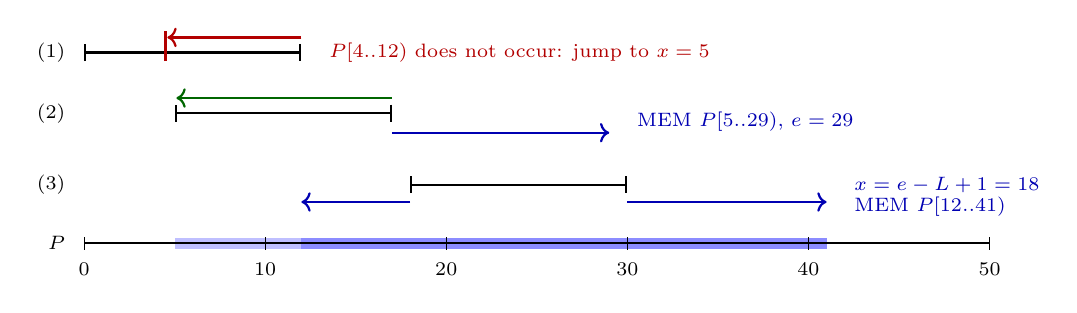
\begin{tikzpicture}[x=2.3mm, y=5.5mm, every node/.style={font=\scriptsize}]
\fill[blue!25] (5,-0.13) rectangle (29,0.13);
\fill[blue!45] (12,-0.13) rectangle (41,0.13);
\draw[thick] (0,0) -- (50,0); \node[anchor=east] at (-0.5,0) {$P$};
\foreach \i in {0,10,20,30,40,50} { \draw (\i,-0.15) -- (\i,0.15); \node[below=2pt] at (\i,-0.1) {\i}; }
\node[anchor=east] at (-0.5,4.4) {(1)};
\draw[|-|, thick] (0,4.4) -- (12,4.4);
\draw[->, red!70!black, thick] (12,4.75) -- (4.6,4.75); \draw[red!70!black, thick] (4.5,4.2) -- (4.5,4.9);
\node[red!70!black, anchor=west] at (13,4.4) {$P[4..12)$ does not occur: jump to $x = 5$};
\node[anchor=east] at (-0.5,3.0) {(2)};
\draw[|-|, thick] (5,3.0) -- (17,3.0);
\draw[->, green!40!black, thick] (17,3.35) -- (5.1,3.35);
\draw[->, blue!70!black, thick] (17,2.55) -- (29,2.55);
\node[blue!70!black, anchor=west] at (30,2.8) {MEM $P[5..29)$, $e = 29$};
\node[anchor=east] at (-0.5,1.35) {(3)};
\draw[|-|, thick] (18,1.35) -- (30,1.35);
\draw[->, blue!70!black, thick] (18,0.95) -- (12,0.95);
\draw[->, blue!70!black, thick] (30,0.95) -- (41,0.95);
\node[blue!70!black, anchor=west] at (42,1.35) {$x = e - L + 1 = 18$};
\node[blue!70!black, anchor=west] at (42,0.85) {MEM $P[12..41)$};
\end{tikzpicture}
\caption{Boyer--Moore--Li with $L = 12$ on a pattern $P$.
(1)~The search for the window $P[0..12)$ fails at the step that prepends $P[4]$, so no MEM of length at least $L$ starts at positions 0 to 4, and BML jumps to $x = 5$.
(2)~The window $P[5..17)$ occurs; it cannot be extended to the left, since $P[4..17)$ contains $P[4..12)$, so BML extends it to the right and reports the MEM $P[5..29)$.
(3)~The next window is $P[18..30)$; BML extends it in both directions, to the MEM $P[12..41)$, and continues with $x = 30$.}
\label{fig:bml}
\end{figure}

\subparagraph*{Longest MEMs.}
BML can also find the longest MEMs of a pattern in one pass, without a threshold: start with $L = 1$ and, whenever a MEM longer than $L$ is found, set $L$ to its length.
Raising $L$ only stops the search for MEMs shorter than one already found, and a MEM as long as the current $L$ is still found, so the longest MEMs, including ties, are among those reported; as $L$ grows, BML skips more of the pattern.
We call this \emph{BML with adaptive $L$}.
The experimental appendix of the full version of Gagie's BML paper~\cite{Gag24arxiv} already found a longest MEM this way, keeping $L$ one more than the length of the longest MEM found so far; keeping $L$ equal to that length also reports ties.

\subparagraph*{KeBaB.}
KeBaB~\cite{BrownEtAl2025KeBaB} first cuts a pattern into \emph{pseudo-MEMs}, the maximal substrings of length at least $k$ all of whose $k$-mers pass a Bloom filter of the $k$-mers of $T$, so that every MEM of length at least $k$ lies in a pseudo-MEM and only the pseudo-MEMs need to be searched.

% zymo.tex -- owner: KATKA task.
% Extracted by the merging task (2026-10-30) from tax_cpm.tex: the Zymo part of Section 3,
% "Which matches: Zymo" in Section 4, "The index", "Long, noisy reads" and "Longest MEMs" in Section 5,
% and Zymo in Section 7.  Key map and renamings applied (see NOTES.md).  Lines marked %MERGE were added
% or rewritten by the merging task; please check them.
\section{Long noisy reads: finding the right matches}
\label{sec:zymo}
\label{sec:regimes}
\label{sec:setup}

%MERGE
Our first experiment classifies long, noisy reads from whole bacterial genomes to species.
Almost every long MEM occurs in one species, so how a MEM splits its credit among the taxa containing it (Section~\ref{sec:schemes}) hardly matters; what matters is finding the right matches, which errors break and low-complexity regions imitate.

\subparagraph*{Data.}
SPUMONI~2's experiments~\cite{AhmedEtAl2023} use ONT reads of a ZymoBIOMICS \emph{mock community}, a laboratory mixture of known bacteria and yeasts, with a reference of 14\,280 RefSeq sequences of seven of its bacterial species, from 267 for \emph{B.~subtilis} to 7\,914 for \emph{E.~coli}, and minimap2 alignments to label each read with a species or as yeast.
N.~Brown made the reference, the reads and their labels available.\footnote{\url{https://zenodo.org/records/23251764}}
There are 581\,802 bacterial reads with a species label, which we classify whole.
SPUMONI~2's Table~2 instead takes the first 180 to 720 bases of each of these reads and of 10\,245 yeast reads, and asks whether each prefix comes from the bacterial reference; the \emph{sensitivity} is the fraction of bacterial reads that are accepted, and the \emph{specificity} the fraction of yeast reads that are rejected.
Here a taxon contains many complete genomes, which are long and close to each other, the reads are long but have frequent errors, especially in homopolymers, and some reference sequences contain long low-complexity regions, such as the short repeats at the ends of yeast chromosomes (telomeres).
%MERGE: machine sentence split from KATKA's "Machines" paragraph
We ran this experiment on a two-year-old laptop (Intel Core i5-1335U, 12 threads, 14\,GB of RAM available); our numbers for SPUMONI~2 and minimap2 are from their papers.

\subparagraph*{The index.}
\label{sec:index}
For $i = 1, \ldots, d$, let $G_i$ be the concatenation of the reference sequences of taxon $i$, separated by a character \texttt{X} that matches nothing, with the taxa numbered in the left-to-right order of the leaves of the taxonomy.
We index the text $T = G_1 \mathtt{X}\, \mathrm{rc}(G_1) \mathtt{X} \cdots G_d \mathtt{X}\, \mathrm{rc}(G_d) \mathtt{\$}$ of length $n$, where $\mathrm{rc}$ denotes the reverse complement and \texttt{\$} is the terminator; no match crosses a separator.
We call $G_i \mathtt{X}\, \mathrm{rc}(G_i) \mathtt{X}$ the \emph{segment} of taxon $i$ (for $i = d$, the last character is the terminator).
The \emph{tag array} $\mathcal{T}[0..n)$ gives, for each row $i$, the taxon $\mathcal{T}[i]$ of the segment containing $\mathrm{SA}[i]$ (Section~\ref{sec:tags}).
We store the BWT of $T$ as an explicit RLCSA (Section~\ref{sec:prelim}).
As Bowtie~2~\cite{LS12} and Cliffy do, we also store the BWT interval of every string of length $k_t = 10$, so that a search starts with one table lookup; if the string does not occur, we fall back to stepping base by base, so we still know exactly where a match fails.
Here we tag each suffix of $T$ with its species.
Tagging each suffix with its genome instead, which would make $T$ a collection of documents in the usual sense, gives a tag array with too many runs (Section~\ref{sec:tags}).
We homopolymer-compress the reference and the reads (below), after which $T$ has $n = 39.3$ billion characters and its BWT has $r = 338$ million runs, against $n = 53.7$ billion and $r = 437$ million without compression.
We count a read as correct if its species alone has the largest weight.
Our implementation, KATKA, is in the directory \texttt{katka} of \url{https://github.com/TravisGagie/MEM-finding}.

\subparagraph*{Long, noisy reads.}
\label{sec:bml}
ONT reads have many errors in \emph{homopolymers}, runs of a repeated base, and these errors break long matches.
We therefore \emph{homopolymer-compress} the reference and each read, replacing every run of equal bases by a single base, and measure $L$ in compressed characters ($L = 30$ is about 41 bases on the Zymo reads); spans are mapped back to the read's coordinates for scoring.
Homopolymer compression also turns some low-complexity sequences into short periodic ones: yeast telomeric repeats become nearly $(\mathtt{CA})^*$, and AT-rich regions of mitochondrial DNA nearly $(\mathtt{TA})^*$.
Long MEMs in such regions occur in many places, and mostly in the reference genomes of a few species, so they pull reads towards those species.
We therefore ignore every MEM with fewer than $\theta$ distinct 3-mers, computed on the compressed sequence; we use $\theta = 14$, out of the 36 3-mers without repeated consecutive bases.
On the 720-base Zymo prefixes, this raises the specificity of the test of SPUMONI~2's Table~2 from 89.18\% to 97.90\% at the cost of 0.03 points of sensitivity; without homopolymer compression (and $\theta = 16$ of 64), the test gives 97.24\% and 97.98\%, so compression mainly makes the index smaller ($r = 338$ instead of 437 million).

\subparagraph*{Longest MEMs.}
%MERGE: the description of BML with adaptive L moved to the preliminaries
We find the longest MEMs of each read with BML with adaptive $L$ (Section~\ref{sec:prelim}).
Searching only the longest pseudo-MEMs of KeBaB (Section~\ref{sec:prelim}), as in KeBaB's pipeline, can miss the longest MEM, since a long pseudo-MEM need not contain one; instead, as Brown et al.\ suggest~\cite{BrownEtAl2025KeBaB}, we search the pseudo-MEMs from longest to shortest and stop at the first one shorter than the current $L$, which loses nothing. %MERGE: credit to KeBaB for the idea (KATKA Appendix C cites it)
On the 581\,802 whole Zymo reads, this finds exactly the same longest MEMs as without the filter, which takes 0.135\,GB, and classification takes 118\,s with 12 threads on the laptop, against 211\,s without the filter and about 780\,s with $L = 30$; on SILVA, whose short, accurate reads have almost all their $k$-mers in the database, the filter saved little time (Appendix~\ref{app:alternatives}).
%MERGE: caveat agreed by both tasks (brief, "Things not to claim")
This speed-up comes from the filter and the longest-first stopping rule; we have not compared our MEM-finding alone with Tagger, ropebwt3 or Movi~2 on these reads.

\subparagraph*{Which matches.}
\label{sec:zymo-accuracy}
On the Zymo reads, $L = 30$ homopolymer-compressed characters (about 41 bases) is the best fixed threshold (99.43\% with proportional credit), since ONT reads have few error-free stretches much longer.
Even so, 0.4\% of the reads have no MEM that long and stay unclassified.
Using only the longest MEMs of each read, measured in compressed characters, every read is classified, and proportional credit reaches 99.61\%, the best of all our configurations; on the 720-base prefixes, species accuracy is 97.88\% with proportional credit and 97.44\% with even credit.
How the credit is split hardly matters: the 89.6 million long MEMs of the whole reads occur in 1.01 species on average, and all the schemes of Table~\ref{tab:credit} are within 0.16 percentage points (\emph{points}, from now on) of each other: the sample reaches 99.58\%, even credit and the range 99.54\%, and proportional credit 99.43\%, and normalising each count by the number of reference sequences of its species, or by their total length, gives 99.42\% and 99.43\%.

In the prefix test of SPUMONI~2's Table~2 with the first 720 bases of each read, we have 97.24\% sensitivity and 97.98\% specificity without homopolymer compression (96.88\% and 97.90\% with it), against 95.32\% and 97.06\% for SPUMONI~2 with minimizer digests, 97.62\% and 97.38\% for SPUMONI~2 without them, and 97.90\% and 97.85\% for minimap2.
With the longest MEMs, thresholding their length gives a whole sensitivity--specificity curve from one run: with homopolymer compression, 97.32\% and 96.33\% at 28 compressed characters, and 96.88\% and 97.90\% at 30.
The longest MEMs of yeast prefixes have a median of 23 compressed characters, about $\log_4$ of $n$ times the prefix length, as for random strings, so the threshold can be set a few characters above that rather than tuned.

\subparagraph*{Time and space.}
For the homopolymer-compressed Zymo reference, the tag array takes 1.47\,GB, an RLBWT 1.00\,GB and an explicit 64-bit RLCSA 5.56\,GB; with the RLCSA and the longest MEMs we classify 4\,900 whole reads per second with 12 threads on the laptop (peak memory 8.0\,GB).
The prefix test needs no tags, and with the RLBWT alone takes 109\,s for the 720-base prefixes, against the 194\,s and 0.74 to 1.54\,GB that SPUMONI~2 reports on its machine.

% silva.tex -- owner: KATKA task.
% Extracted by the merging task (2026-10-30) from tax_cpm.tex: Section 2 (matches and credit schemes,
% Table 1, Figure 1), the SILVA part of Section 3, "Which credit: SILVA" in Section 4, Section 6 (tag
% arrays) and SILVA in Section 7.  Key map and renamings applied (see NOTES.md).  Lines marked %MERGE
% were added or rewritten by the merging task; please check them.
\section{Short reads, many taxa: answering each MEM}
\label{sec:silva}

%MERGE
Our second experiment classifies short 16S rRNA reads to genera.
Long MEMs are still the right matches, but many of them occur in several genera, so the bottleneck is answering each MEM: deciding how it splits its credit among the taxa containing it, and computing what that split needs.

\subsection{Matches and credit}
\label{sec:schemes}
\label{sec:background}

\subparagraph*{Matches.}
%MERGE: the definition of MEMs moved to the preliminaries
Let $T$ be the reference text, consisting of the reference sequences and their reverse complements, grouped by taxon as in Section~\ref{sec:index}, and let $P$ be a read.
We use the MEMs of $P$ (Section~\ref{sec:prelim}), as Tagger does.
Cliffy instead cuts the read into consecutive \emph{Ziv--Merhav phrases} (ZMPs) by searching backward from the end of the read for as long as the match occurs, and starting a new search at the character where the previous one failed.
This mirrors the cross parsing of Ziv and Merhav~\cite{ZM93}, later used as Relative Lempel--Ziv (RLZ) parsing~\cite{KPZ10}.
Each ZMP $P[j..f)$ is the longest suffix of $P[0..f)$ that occurs in $T$, so it cannot be extended to the left and is a prefix of the MEM starting at $j$; ZMPs are generally shorter than the MEMs that contain them.
A $k$-mer is a substring of fixed length $k$, and Kraken~2 uses minimizers: from each $k$-mer it keeps the substring of a fixed shorter length with the smallest hash.
Short matches occur in many taxa, so they say little about where a read came from; with Boyer--Moore--Li we use only the MEMs of length at least a threshold $L$.

\subparagraph*{Credit.}
Let $M$ be a match, let $c_g$ be the number of occurrences of $M$ in the reference sequences of taxon $g$, counting both strands, let $D = \{g : c_g > 0\}$ and let $C = \sum_g c_g$.
A \emph{credit scheme} splits the credit $|M|$ into weights $w_v \geq 0$ for the nodes $v$ of the taxonomy, with $\sum_v w_v = |M|$; all schemes except Kraken~2's give weight only to the leaves, which are the taxa we classify to.
The read is assigned to the taxon with the largest total weight over all its matches, except with Kraken~2's scheme.
Table~\ref{tab:schemes} lists the schemes we consider, with the $d$ taxa numbered $1, \ldots, d$ in the left-to-right order of the leaves of the taxonomy, so that the taxa under any node form an interval, and with $g_\ell = \min D$ and $g_r = \max D$.
\begin{description}
\item[LCA.] Kraken~2 gives $|M|$ to the LCA of $D$, and assigns the read to the leaf whose root-to-leaf path collects the most weight.
Cliffy's LCA query instead splits the credit evenly over the \emph{range} of taxa from $g_\ell$ to $g_r$, giving $|M|/(g_r - g_\ell + 1)$ to each, including taxa that do not contain $M$; all of them lie under the LCA.
\item[One label per position.] For each position of the read, SPUMONI~2 computes the length of the longest match starting there (the matching statistics, approximated), with the r-index~\cite{GagieNavarroPrezza2020}, and for classification into several classes the class of one occurrence of that match, read from document-array samples at the boundaries of BWT runs~\cite{AhmedEtAl2023}; the read goes to the class with the most positions.
\item[One label per MEM.] Tagger gives $|M|$ to the taxon of the last occurrence of $M$ in BWT order, which it maintains during the search much as the r-index maintains its \emph{toehold}, the position of one occurrence of the current match.
That occurrence is more likely to lie in a taxon with many occurrences, so we model this scheme as giving $|M|$ to one taxon $g$ drawn with probability $c_g / C$, although Tagger's label is deterministic.
\item[Sample.] Cliffy's approximate document listing gives $|M|/|D'|$ to each taxon of a subset $D' \subseteq D$.
At the boundaries of BWT runs, Cliffy stores a \emph{document array profile}~\cite{ARBL23}, which gives for each taxon the length of the longest common prefix of the suffix at that position with any suffix of that taxon, and keeps only its \emph{cliffs}: the entries larger than every entry to their left, or to their right, in the order of the taxa.
These are left-to-right and right-to-left maxima, or records (B.~Langmead, personal communication), and a random permutation of $d$ distinct values has on average $H_d = \ln d + O(1)$ left-to-right maxima~\cite{Ren62}, so there are often about logarithmically many cliffs.
$D'$ consists of the taxa whose cliffs are at least $|M|$, so it is determined by the order of the taxa, not drawn at random or weighted by counts, and it always contains $g_\ell$ and $g_r$.
\item[Even.] Each taxon in $D$ gets $|M|/|D|$, as Cliffy's approximate document listing would if it listed $D$ exactly.
\item[Proportional.] Each taxon in $D$ gets $|M| \cdot c_g / C$.
\end{description}

\begin{table}[t]
\centering
\caption{Matches and credit schemes. $M$ is a match, $c_g$ is the number of its occurrences in taxon $g$, $C = \sum_g c_g$, $D$ is the set of taxa containing it, and $g_\ell$ and $g_r$ are the leftmost and rightmost of them in the order of the leaves of the taxonomy.}
\label{tab:schemes}
\resizebox{\textwidth}{!}{\begin{tabular}{llll}
\toprule
classifier & matches & credit scheme & weights \\
\midrule
Kraken~2~\cite{WLL19} & $k$-mers (minimizers) & LCA & $|M|$ to $\mathrm{LCA}(D)$ \\
SPUMONI~2~\cite{AhmedEtAl2023} & longest match at each position & one label per position & -- \\
Tagger~\cite{DAF+25} & MEMs of length $\geq L$ & one label per MEM & $|M|$ to one $g \in D$ \\
Cliffy~\cite{ABL25}, LCA query & ZMPs & range & $|M| / (g_r - g_\ell + 1)$ to each of $g_\ell..g_r$ \\
Cliffy~\cite{ABL25}, approx.\ listing & ZMPs & sample & $|M|/|D'|$ to each of $D' \subseteq D$ \\
-- & MEMs of length $\geq L$ & even & $|M|/|D|$ to each of $D$ \\
ours & MEMs of length $\geq L$ & proportional & $|M| \cdot c_g / C$ to each $g \in D$ \\
\bottomrule
\end{tabular}}
\end{table}

\subparagraph*{Why proportional credit.}
If one label is drawn uniformly at random from the occurrences of $M$, taxon $g$ gets it with probability $c_g / C$, so proportional credit gives each taxon the expected weight of such a draw.
Summed over the matches of a read, proportional credit keeps the expected total weight of each taxon under one label per match, without the variance of the draws, which matters most for reads with few long matches.
Similarly, even credit gives each taxon the expected weight of a label drawn uniformly from $D$.
A sample like Cliffy's is not a uniform subset of $D$, since it always contains $g_\ell$ and $g_r$, so it only roughly approximates even credit.
For a single match, $|M| \cdot c_g / C$ is also $|M|$ times the posterior probability that a string containing $M$ was drawn from taxon $g$, if it was drawn from a uniformly random position of the database, ignoring the boundaries of the sequences and overlapping occurrences of $M$.
The implicit prior is thus proportional to the amount of sequence of each taxon in the database, and summing over the matches of a read is a heuristic; it does not give the posterior given all the matches.
This prior can help when the taxa that are abundant in the sample also have much sequence in the database, and hurt when they do not; then normalising each count by the size of its taxon, or correcting towards a known or estimated composition of the sample, may be better.

Even credit needs the set $D$ itself, not just $g_\ell$ and $g_r$, and proportional credit needs the counts, which matter when a match occurs much more often in some taxa than in others (Figure~\ref{fig:lca}).

\begin{figure}[t]
\centering
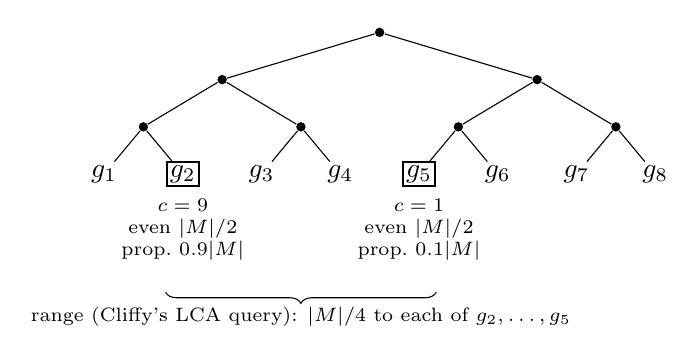
\begin{tikzpicture}[level distance=6mm, every node/.style={inner sep=1.2pt},
  level 1/.style={sibling distance=40mm}, level 2/.style={sibling distance=20mm}, level 3/.style={sibling distance=10mm}]
\node[circle,fill] {}
  child {node[circle,fill] {}
    child {node[circle,fill] {} child {node (g1) {$g_1$}} child {node[draw,thick] (g2) {$g_2$}}}
    child {node[circle,fill] (lca) {} child {node (g3) {$g_3$}} child {node (g4) {$g_4$}}}}
  child {node[circle,fill] {}
    child {node[circle,fill] {} child {node[draw,thick] (g5) {$g_5$}} child {node (g6) {$g_6$}}}
    child {node[circle,fill] {} child {node (g7) {$g_7$}} child {node (g8) {$g_8$}}}};
\node[below=1mm of g2, font=\scriptsize, align=center] {$c = 9$\\even $|M|/2$\\prop.\ $0.9|M|$};
\node[below=1mm of g5, font=\scriptsize, align=center] {$c = 1$\\even $|M|/2$\\prop.\ $0.1|M|$};
\draw[decorate, decoration={brace, mirror, amplitude=4pt}] ([yshift=-15mm]g2.west) -- ([yshift=-15mm]g5.east) node[midway, below=4pt, font=\scriptsize] {range (Cliffy's LCA query): $|M|/4$ to each of $g_2, \ldots, g_5$};
\end{tikzpicture}
\caption{A match $M$ that occurs 9 times in taxon $g_2$ and once in $g_5$ (boxed).
The LCA of $g_2$ and $g_5$ is the root, so with Kraken~2's scheme the match gives weight only to the root.
Cliffy's LCA query splits the credit $|M|$ evenly over the taxa from the leftmost to the rightmost one containing the match, including $g_3$ and $g_4$, which do not contain it.
Even credit splits the credit between $g_2$ and $g_5$, and proportional credit gives $g_2$ nine times as much weight as $g_5$.}
\label{fig:lca}
\end{figure}

Other r-index classifiers, such as SPUMONI~2 and col-BWT~\cite{BrownEtAl2026}, mostly decide whether a read comes from a target pangenome; Cobas, M\"akinen and Rossi~\cite{CMR20} report document frequencies from a grammar-compressed document array; and Omri et al.~\cite{OSM+26} classify genomic sequences by compression.

\subsection{Data}
\label{sec:silva-data}

Many studies of bacterial and archaeal communities sequence only copies of the 16S ribosomal RNA gene, which is about 1\,500 bases long and present in every bacterium and archaeon.
An experiment copies one or two of its nine \emph{hypervariable regions}, V1 to V9, which differ between taxa, and sequences each copy from both ends, giving two reads, or \emph{mates}; the reads are short and the regions similar across related taxa, so 16S reads are usually classified only to genera~\cite{JSL+19}.
We reproduced Cliffy's SILVA experiment~\cite{ABL25} as closely as we could from its authors' scripts.
We used SILVA 138.1 SSU NR99~\cite{QPY+13}, grouped its sequences by genus with their script, and kept 9\,118 genera containing 402\,378 sequences, in the left-to-right order of the leaves of the SILVA taxonomy.
The database is much smaller than the Zymo reference, but the genera are very unevenly represented, and sequences of different genera often share long substrings, which makes classification with exact matches hard and the database very repetitive.
With both strands, $T$ has $n = 1.17$ billion characters and its BWT has $r = 68.3$ million runs.
We simulated 10 million pairs of 250-base reads for each of the regions V1--V2, V3--V4, V4 and V4--V5 with the authors' simulator, MicrobeMixer, using the sequencing-error simulator ART~\cite{HLMM12} and the genus abundances of an aquatic community, and measured accuracy on every 50th pair.
Each mate is classified separately and the weights of the two mates are added; a read pair is \emph{strictly} correct if its true genus alone has the largest weight; ties and unclassified pairs count as wrong.
Cliffy's scoring also counts ties for the largest weight as correct, and pairs without any match unless their genus is ``uncultured'' (a placeholder for sequences not assigned to a known genus).
We report the strict accuracy unless stated otherwise, as the mean over the four regions.
%MERGE: machine sentences split from KATKA's "Machines" paragraph
We used a seven-year-old desktop (Intel Core i7-8700, 6 cores, 16\,GB of RAM) for SILVA.
Cliffy's indexes do not fit on it, so the second author built and ran them, and our default configuration, on our reads on a server with 256\,GB of RAM (Appendix~\ref{app:details}).

\subsection{Which credit}
\label{sec:accuracy}

On SILVA, a long MEM of one of our reads occurs in 3.8 genera on average (Section~\ref{sec:tags}), so the split matters.
Long MEMs are still the right matches.
With the range scheme, all the MEMs of each read were 0.4 to 1.3 points more accurate than ZMPs, both on the sequences and on their \emph{minimizer digests}~\cite{RHH+04,AhmedEtAl2023} (Appendix~\ref{app:matches}).
With even credit, strict accuracy is 90.56\% with $L = 15$ and 90.28\% with $L = 30$, drops by about 2 points at $L = 50$ and collapses for larger $L$, as the 250-base reads start to have no MEM that long (Table~\ref{tab:L}); with proportional credit it is 93.74\% with $L = 15$, 93.77\% with $L = 30$ and 93.48\% with $L = 40$.
Discarding short MEMs also makes classification much faster (Section~\ref{sec:tradeoffs}).

Table~\ref{tab:credit} compares the credit schemes on the same long MEMs, so that only the split differs.
For one label per MEM and for the sample, we simulate the schemes of Tagger and Cliffy from the counts: one label drawn with probability $c_g/C$, and the left-to-right and right-to-left maxima of random values given to the taxa in $D$, which form a sample containing $g_\ell$ and $g_r$ with $2 H_{|D|} - 1$ taxa on average.
The tools themselves give answers that are not random, and use different matches, so this comparison measures the credit schemes, not the tools.
One label drawn by counts is 1.6 points less accurate than proportional credit, which has the same expected weights, so this is roughly what the variance of one label per MEM costs; it is still 1.9 points more accurate than even credit.
The sample is about as accurate as even credit, and both are 3.3 to 3.5 points less accurate than proportional credit.
Proportional credit also almost eliminates ties, and it is 1 point more accurate than normalising each count by twice the number of sequences in the genus, which gives each genus credit in proportion to the fraction of its sequences containing the match.
Even credit is more accurate than the range: with $L = 15$, by 3.5 points without digestion and 3.6 points with it (Appendix~\ref{app:matches}).
On the same machine and reads, Kraken~2 and Tagger are less accurate than long MEMs with proportional credit (Table~\ref{tab:others}).

\begin{table}[t]
\centering
\caption{Accuracy of the credit schemes on the same long MEMs ($L = 30$): species level on the Zymo reads (whole homopolymer-compressed reads, low-complexity MEMs ignored), and genus level on SILVA (strict, mean over the four regions, 200\,000 read pairs per region). One label per MEM and the sample simulate Tagger's and Cliffy's schemes from the counts.}
\label{tab:credit}
\small
\begin{tabular}{lcc}
\toprule
credit scheme & Zymo (species) & SILVA (genus) \\
\midrule
range (Cliffy's LCA query) & 99.54\% & 87.0\% \\
one label per MEM (drawn by counts) & 99.44\% & 92.18\% \\
sample (simulated cliffs) & 99.58\% & 90.47\% \\
even & 99.54\% & 90.28\% \\
proportional, normalised by taxon size & 99.42\% & 92.76\% \\
proportional & 99.43\% & 93.77\% \\
\bottomrule
\end{tabular}
\end{table}

\subparagraph*{Composition.}
MicrobeMixer chooses the genus of each simulated read according to the abundances of an aquatic community, and only then a sequence of that genus, so our SILVA reads are not drawn in proportion to how well each genus is represented in SILVA.
Proportional credit is still the most accurate, and its 1-point advantage over normalised credit suggests that its prior is an advantage here, presumably because genera that are abundant in the community are also well represented in SILVA.

\subsection{Counting with complete tag arrays}
\label{sec:tags}
\label{sec:freq}

\subparagraph*{Tag arrays.}
A tag array associates a tag with each row of the BWT~\cite{BalazEtAl2024,EskandarEtAl2025,ESP26,OO26}, and Wheeler maps~\cite{BalazEtAl2024} bound its space in terms of the number of runs in the tags.
Here the tag array is $\mathcal{T}$, in which the tag of a row is the taxon of the corresponding suffix of $T$.
If a document is the concatenation of the sequences of one taxon, then this tag array is the document array of Muthukrishnan~\cite{Mut02}; other tag arrays, such as those of Eskandar et al.~\cite{EskandarEtAl2025,ESP26}, whose tags are vertices of a pangenome graph, and of Olbrich and Ohlebusch~\cite{OO26}, whose tags are columns of a multiple alignment, are not document arrays.
Tagger~\cite{DAF+25} stores only the tags at the ends of BWT runs, from which the tags of other rows cannot in general be recovered.
To stress the difference, we call a tag array \emph{complete} if it gives the tag of every row, whether it stores them run-length compressed or recovers them from a sample.
We run-length compress the tag array, storing the run starts with Elias--Fano coding and the tag of each run, and let $\rho$ be the number of runs in $\mathcal{T}$, which we call \emph{tag runs}.

\subparagraph*{Contextual locality.}
The runs are few because the BWT sorts the suffixes of $T$, and with them the characters preceding them, by their \emph{contexts}, the strings that follow those characters.
A property has \emph{contextual locality}~\cite{Gagie2024tags,BalazEtAl2024,OO26} if suffixes that share long prefixes tend to have the same value of the property, their tag.
Olbrich and Ohlebusch~\cite{OO26} note that the tag array of such a property is then likely to be run-length compressible, for the same reason that the BWT of a repetitive text is; Lemma~\ref{lem:runs} makes this precise for tags that are constant on segments of $T$, such as taxa.
Let a \emph{tag boundary} be a row $p > 0$ with $\mathcal{T}[p - 1] \neq \mathcal{T}[p]$, so that $\rho$ is one more than the number of tag boundaries, and let $\mathrm{lcp}(p)$ be the length of the longest common prefix of the suffixes starting at $\mathrm{SA}[p - 1]$ and $\mathrm{SA}[p]$.
A tag boundary $p$ with a large $\mathrm{lcp}(p)$ is a violation of contextual locality: two suffixes with a long common prefix but different tags.

\begin{lemma}
\label{lem:runs}
Let $T[0..n)$, over an alphabet of size $\sigma$ and ending with a unique terminator, be cut into $d$ segments, each with a tag, let $\mathcal{T}[i]$ be the tag of the segment containing $\mathrm{SA}[i]$, and let $r$ be the number of runs in the BWT of $T$.
For any $\lambda \geq 0$, if $B_\lambda$ is the number of tag boundaries $p$ with $\mathrm{lcp}(p) > \lambda$, then $\rho \leq (r + \sigma + 2d)(\lambda + 1) + B_\lambda + 1$.
\end{lemma}

\begin{proof}
Call a row $p > 0$ a \emph{break} if $\Psi(p) \neq \Psi(p - 1) + 1$.
$\Psi$ maps the rows whose suffixes start with a character $c$, in order, to the rows of the occurrences of $c$ in the BWT, so a break is either a row where the first character of the suffixes changes, or one where two consecutive occurrences of $c$ in the BWT are in different runs; there are at most $r + \sigma$ breaks.
Let $p_0$ be a tag boundary with $\mathrm{lcp}(p_0) \leq \lambda$, and while $p_h$ is a tag boundary and not a break, let $p_{h + 1} = \Psi(p_h)$.
Then $\Psi(p_h - 1) = p_{h + 1} - 1$, so the suffixes at rows $p_{h + 1} - 1$ and $p_{h + 1}$ are those at rows $p_h - 1$ and $p_h$ without their first character, which is the same, and $\mathrm{lcp}(p_{h + 1}) = \mathrm{lcp}(p_h) - 1$.
Let $h$ be the largest index such that $p_h$ is a tag boundary.
A row with lcp $0$ is a break, so $h \leq \mathrm{lcp}(p_0) \leq \lambda$.
Either $p_h$ is a break, or $p_{h + 1}$ is not a tag boundary although $p_h$ is, which means that one of $\mathrm{SA}[p_h - 1]$ and $\mathrm{SA}[p_h]$ is the last position of a segment; each of the $d$ last positions is $\mathrm{SA}[q]$ for one $q$, and then $p_h \in \{q, q + 1\}$, so there are at most $2d$ such rows $p_h$.
Since $p_0 = \mathrm{LF}^h(p_h)$, the pair $(p_h, h)$ determines $p_0$, so there are at most $(r + \sigma + 2d)(\lambda + 1)$ tag boundaries with lcp at most $\lambda$.
Adding the $B_\lambda$ other tag boundaries, and 1 because $\rho$ is one more than the number of tag boundaries, gives the bound.
\end{proof}

$B_\lambda$ itself measures violations of contextual locality, so the content of the lemma is that all the other tag boundaries number $O((r + \sigma + d)(\lambda + 1))$, independently of $n$: $\rho$ is small when $r$ and $d$ are small and, for some modest $\lambda$, few suffixes adjacent in suffix-array order share a prefix longer than $\lambda$ but have different tags.
In a reference with many genomes per species, we expect nearly every suffix to share a longer prefix with the corresponding suffixes of other genomes of its species than with any suffix of another species, so that species have contextual locality.
On the homopolymer-compressed Zymo reference, $\rho = 449$ million, only 1.33 times $r$.
If each genome is instead its own tag, the tag array is a document array, and corresponding suffixes of the genomes of a species, which are adjacent in suffix-array order and share long prefixes, have different tags, so $B_\lambda$ is large for any modest $\lambda$ and Lemma~\ref{lem:runs} gives no useful bound; in practice that tag array had so many runs that its construction ran out of memory.
On SILVA, $\rho = 359$ million, 5.3 times $r$, presumably because 16S sequences of different genera often share long substrings.

\subparagraph*{Counting.}
To count the occurrences of a MEM in each taxon, we scan the runs that overlap the MEM's BWT interval and add up the lengths of the runs of each taxon, clipped to the interval.
After a predecessor search for the first run, this takes time proportional to the number of runs in the interval rather than to the number of occurrences, and never locates an occurrence.
When counts are not needed, Muthukrishnan's document listing algorithm~\cite{Mut02} lists the taxa in an interval in time proportional to their number, with a range-minimum structure~\cite{FH11} over the array that points from each run to the previous run with the same tag; as in Sadakane's method~\cite{Sad07} and as Olbrich and Ohlebusch do~\cite{OO26}, that array need not be stored.
The usual alternative is to locate every occurrence with an r-index~\cite{GagieNavarroPrezza2020}, from the toehold with $\phi$ queries, and map each to its taxon with a predecessor search over the taxon starts.
This also gives exact counts, but costs a $\phi$ query, with its cache misses, for every occurrence.
On SILVA the difference is large, because genera contain many near-identical sequences: a MEM of at least 30 bases in one of our reads occurs 70 times on average, in 3.8 genera; half of these MEMs occur only once and 5\% occur more than 200 times, yet their BWT intervals contain few tag runs.
With the same RLCSA and lookup table, classifying with an r-index takes 125\,$\mu$s per read, against 66\,$\mu$s with the tag array, for an index only 0.06\,GB smaller.

\subparagraph*{Construction.}
The tag array needs no suffix array.
One pass of LF over the text gives the suffix-array samples at the BWT run boundaries, as for the r-index, and from them $\phi$ streams the suffix array from the last row to the first; each entry is mapped to its taxon with a predecessor search, and consecutive positions with the same taxon are merged into runs, which are written to disk as they are completed.
The memory needed is therefore proportional to $r + d$, plus $\rho$ for reading the runs back.
On SILVA this takes about 6 minutes and 3.3\,GB on the desktop, and on the homopolymer-compressed Zymo reference 7.2 hours and 8.9\,GB on the laptop (with a version of the construction that kept all the runs in memory).

\subparagraph*{Grammar-compressing the runs.}
\label{sec:grammar}
Our default configuration uses only run-length compression, but the sequence of the runs' tags can be compressed further.
LF maps the rows $i..j$ of a BWT run to consecutive rows $\mathrm{LF}(i)..\mathrm{LF}(j)$, whose suffixes are one character longer, so the tags at rows $\mathrm{LF}(i)..\mathrm{LF}(j)$ are a copy of those at rows $i..j$, except at the rows $\mathrm{LF}(q)$ such that $\mathrm{SA}[q]$ is the first position of a segment.
The copying holds because the tag of a suffix does not change when the suffix is extended by one character within its segment.
It fails for tag arrays in general: the BWT itself is a tag array, in which each suffix is tagged with the character preceding it, and it is run-length compressible, but LF does not map its runs to copies of themselves.

\begin{observation}
\label{obs:grammar}
Let $T[0..n)$, ending with a unique terminator, be cut into $d$ segments, each with a tag, let $\mathcal{T}[i]$ be the tag of the segment containing $\mathrm{SA}[i]$, and let $r$ be the number of runs in the BWT of $T$.
Then $\mathcal{T}$ has a bidirectional macro scheme with at most $r + 2d$ phrases, and therefore a string attractor of size at most $r + 2d$ and a grammar of size $O((r + d) \log (n / (r + d)))$.
\end{observation}

\begin{proof}
Unless $\mathrm{SA}[q]$ is the first position of a segment, $\mathcal{T}[\mathrm{LF}(q)] = \mathcal{T}[q]$, since $\mathrm{SA}[\mathrm{LF}(q)] = \mathrm{SA}[q] - 1$ is in the same segment (taking positions cyclically, so that $\mathrm{SA}[\mathrm{LF}(q)] = n - 1$ when $\mathrm{SA}[q] = 0$).
Let $\mathcal{T}[p]$ copy $\mathcal{T}[\Psi(p)]$ for every such row $p = \mathrm{LF}(q)$, and store $\mathcal{T}[p]$ explicitly at the other $d$ rows, at which $\mathrm{SA}[p]$ is the last position of a segment.
LF maps the rows of each BWT run to consecutive rows, in order, so cutting $[0..n)$ at the ends of the images of the $r$ runs and around the $d$ explicit rows gives at most $r + 2d$ phrases, each a copy of a substring of $\mathcal{T}$ or a single explicit symbol.
Following copies from any row $p$ moves to $\Psi(p)$, whose suffix starts one position later in $T$, so it reaches an explicit row before leaving the segment containing $\mathrm{SA}[p]$, and the scheme is a valid bidirectional macro scheme.
The size $\gamma$ of the smallest string attractor of a string is at most the number of phrases of any bidirectional macro scheme for it, and the string has a grammar of size $O(\gamma \log (n/\gamma))$~\cite{KP18}; since $x \log (n/x)$ is increasing for $x \leq n/e$ and $\gamma \leq r + 2d$, the bound follows.
\end{proof}

We say that a property constant on few segments of $T$, such as documents, genomes and taxa, has \emph{textual locality}.
Textual locality gives the macro scheme of Observation~\ref{obs:grammar}, with $O(r + d)$ phrases, while contextual locality gives few runs, by Lemma~\ref{lem:runs}.
The characters themselves have contextual locality but not textual locality, so the BWT is run-length compressible, but LF does not map its runs to copies of themselves.
Taxa have both, so their tag array has few runs and also a macro scheme with at most $r + 2d$ phrases, which is smaller when $\rho \gg r$; genomes, with many per species, have mainly textual locality.
Cobas and Navarro~\cite{CN19} used the copies in the proof of Observation~\ref{obs:grammar} to grammar-compress the document array, as with the differential suffix array~\cite{GN07,GagieNavarroPrezza2020}.
We instead run-length compress first, and grammar-compress only the sequence of the runs' taxa (their lengths come from the run starts), which has length $\rho$ rather than $n$; Observation~\ref{obs:grammar} does not directly bound this grammar.
On SILVA we build the grammar with RePair~\cite{LM00}, in the second author's implementation distributed with BigRePair~\cite{GIM+19}, which avoids deep rules, and encode it as Gagie et al.\ do~\cite{GIM+20}; to count, we find the first run of the interval by a predecessor search on the final sequence, descend through the grammar, and decode the following runs.
The runs' taxa then take 0.23\,GB instead of 0.63\,GB, and the index 1.04\,GB instead of 1.44\,GB, while classification takes 75.0\,$\mu$s per read instead of 66.0, with identical answers.

\subsection{Time and space}
\label{sec:tradeoffs}

Our default index for SILVA takes 1.44\,GB: 0.57\,GB for the RLCSA, 0.86\,GB for the tag array (19.1 bits per run) and 18\,MB for the lookup table.
Building it from the sequences takes minutes on the desktop: 347\,s for the BWT, with prefix-free parsing~\cite{BoucherEtAl2019} (peak memory 5.1\,GB), a few seconds for the RLCSA and the lookup table, and about 6 minutes for the tag array.
With one thread it classifies a read in 66\,$\mu$s, excluding loading the index and reading the reads, and with 12 threads on 6 cores, sharing one copy of the index, 144\,800 reads per second.
Table~\ref{tab:others} compares our index with Kraken~2 and Tagger, run on the same machine and reads, and with Cliffy's LCA query, run on our reads on the server.
There our accuracy for the default configuration is on fewer reads and its time is measured differently, so these numbers differ from those above (Appendix~\ref{app:details}).
On the server, our default index takes 1.42\,GB and 146\,$\mu$s per read and reaches 93.70\%, while Cliffy's undigested index takes 19.58\,GB and its LCA query takes 637\,$\mu$s and reaches 85.75\% (86.45\% with Cliffy's scoring); building it took almost three days, over 2\,TB of temporary disk space and more than 200\,GB of memory.
On Cliffy's digested index, which takes 7.63\,GB, it reaches 84.15\% (85.53\%), against 92.08\% on the server for our digested index, which takes 0.49\,GB.
With Cliffy's scoring, both are up to 4 points below what Cliffy's paper reports for its LCA query on its own reads (87.5 to 90.2\% and 86.3 to 88.5\%), as are the rz-index's results with Cliffy's matches on our reads (Appendix~\ref{sec:rz}), so our reads seem slightly harder; we have not run Cliffy's approximate listing, for which its paper reports 93.3 to 94.8\% and 92.8 to 93.4\%.
Appendix~\ref{app:listing} gives the time--space--accuracy Pareto surface, with indexes down to 0.41\,GB, or 0.16\,GB over minimizer digests.

\begin{table}[t]
\centering
\caption{SILVA: index size, time per read with one thread and reads per second with 12 threads (both excluding loading), and genus-level accuracy (mean over the four regions).
The first, fourth and fifth rows are on the desktop, with accuracy on 5\,000 read pairs per region and time as total time over the number of reads (200\,000 pairs per region); our other rows use the mean of per-read timings (66.0\,$\mu$s for the default) and 200\,000 pairs.
Tagger's three accuracies count pairs with disagreeing mates as wrong, random or correct.
Cliffy's numbers are on our reads (5\,000 pairs per region) and on the server, where our default configuration takes 146\,$\mu$s per read with the same accuracy as here.}
\label{tab:others}
\resizebox{\textwidth}{!}{\begin{tabular}{lrrrc}
\toprule
classifier & space (GB) & time ($\mu$s) & reads/s, 12 threads & accuracy \\
\midrule
long MEMs, proportional credit & 1.44 & 53.1 & 144\,800 & 93.70\% \\
\quad grammar-compressed runs & 1.04 & 75.0 & & \\
\quad minimizer digests & 0.49 & 39.3 & & 92.48\% \\
Kraken~2 & 0.15 & 14.3 & 366\,900 & 79.26\% \\
Tagger & 0.82 & 70.4 & 82\,600 & 81.69 / 87.24 / 92.78\% \\
Cliffy, undigested, LCA query & 19.58 & 636.6 & & 85.75\% \\
Cliffy, digested, LCA query & 7.63 & 419.1 & & 84.15\% \\
\bottomrule
\end{tabular}}
\end{table}

% chr19.tex -- owner: More RLBWT Tricks task.
% Extracted by the merging task (2026-10-30) from paper.tex: Sections 3-7 (Section 5 shrunk to two
% sentences, Table 2 shortened to its 1% rows), with the unitig example and Figure 1 from the
% introduction.  Renamings applied (see NOTES.md).  Lines marked %MERGE were added or rewritten by the
% merging task; please check them.
\section{Long matches: crossing them quickly}
\label{sec:chr19}

%MERGE
Our third experiment finds the MEMs of whole chromosome~19 haplotypes
with respect to collections of 16 to 64 other chromosome~19s
(\Cref{sec:chr19-exp}). Almost every character of such a pattern lies
in a long MEM, so the matches are easy to find and we do not classify
them; the bottleneck is crossing them, since backward search takes one
step per character even when the pattern matches material that occurs
many times in the collection. In this section $T = S_1 \# S_2 \# \cdots \#
S_d \# \$$ is a collection of $d$ genomes over
$\{\texttt{A},\texttt{C},\texttt{G},\texttt{N},\texttt{T}\}$, with $\$
< \# < \texttt{A} < \texttt{C} < \texttt{G} < \texttt{N} <
\texttt{T}$, on the forward strand only, and we index $T$ and the
reversed collection $T'$ (\Cref{sec:prelim}), each with an RLBWT.

Repetitiveness is not only a challenge for indexes built on RLBWTs but also an
opportunity. One reason the $r$-index was surprising is that it locates
the occurrences of a pattern not only in space proportional to $r$ but
also in predecessor time, $O(\log \log_w (n/r))$ per occurrence on a
word RAM with $w$-bit words~\cite{GagieNavarroPrezza2020}, and Nishimoto
and Tabei~\cite{NishimotoTabei2021} reduced this to constant time per
occurrence, still in $O(r)$ words, and backward search to constant time
per step when the alphabet has polylogarithmic size. FM-indexes and
compressed suffix arrays that use $O(n \log \sigma)$ bits access the
suffix array in $O((\log_\sigma n)^\epsilon)$ time, for a constant
$\epsilon > 0$~\cite{FerraginaManzini2000,GrossiVitter2005}, and Kempa and
Kociumaka~\cite{KempaKociumaka2026} recently proved that, for binary
texts in general, constant-time access requires $\Omega(n \log^\epsilon
n)$ bits for some $\epsilon > 0$. On a text that is not repetitive,
$O(r)$ words are $\Theta(n \log n)$ bits, so the comparison makes sense
only because the text is repetitive. Nishimoto and Tabei obtained their
bounds with move structures, which replace the rank queries of backward
search by lookups in a table with one entry per run: for a text that is
not repetitive the table would be huge, but for a pangenome it is
small, and in practice much faster than rank
queries~\cite{ZakeriEtAl2024}. Because pangenomes compress so well, we
have room to store structures that would make no sense for a single
reference, and the door is open to doing things with RLBWTs that we
could not do with BWTs. This paper takes another step in that
direction.

Ben Langmead asked us whether BWT-based indexes could get the kind of
speedup that unitigs give $k$-mer indexes. \Cref{fig:dbg} shows a collection of twelve strings
and its de Bruijn graph for $k = 3$, uncompacted and compacted. Every
string contains the unitig \texttt{AACGCTC}, and ten of them contain
the string \texttt{GTCAAGG}, which would be a unitig if two strings did
not have \texttt{GTCCAGG} instead; we call such a string an
\emph{almost-unitig}. The unitig and the almost-unitig appear in
different orders in different strings, so neither can be extended.
Every occurrence of a unitig's last $k$-mer is preceded by the rest of
the unitig, unless a string starts inside the unitig; in the BWT this means
that the interval of the last $k$-mer is mapped one-to-one, in order,
onto the interval of the whole unitig, so a backward search that reaches
the last $k$-mer of \texttt{AACGCTC} and then reads \texttt{AACG} in the
pattern can cross those four characters in one step. For an
almost-unitig, some rows drop out on the way, and a bitvector over the
interval of the last $k$-mer says which.

\begin{figure}[t]
  \centering
  \small
  \begin{tabular}{@{}l r@{}}
    \texttt{GTA\,AACGCTC\,GTCAAGG\,TGG} & $\times 5$ \\
    \texttt{GTA\,AACGCTC\,GTCCAGG\,TGG} & $\times 1$ \\
    \texttt{GTA\,GTCAAGG\,AACGCTC\,TGG} & $\times 5$ \\
    \texttt{GTA\,GTCCAGG\,AACGCTC\,TGG} & $\times 1$
  \end{tabular}

  \medskip
  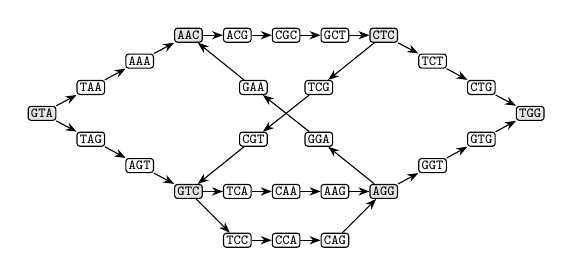
\begin{tikzpicture}[x=0.62cm,y=0.62cm,>={Stealth[length=1.4mm]},v/.style={draw,rounded corners=1pt,inner sep=1pt,font=\tiny\ttfamily}]
\node[v,fill=gray!20] (GTA) at (0.00,0.00) {GTA};
\node[v,fill=gray!20] (AAC) at (3.00,1.60) {AAC};
\node[v,fill=gray!20] (CTC) at (7.00,1.60) {CTC};
\node[v,fill=gray!20] (GTC) at (3.00,-1.60) {GTC};
\node[v,fill=gray!20] (AGG) at (7.00,-1.60) {AGG};
\node[v,fill=gray!20] (TGG) at (10.00,0.00) {TGG};
\node[v] (TAA) at (1.00,0.53) {TAA};
\node[v] (AAA) at (2.00,1.07) {AAA};
\node[v] (TAG) at (1.00,-0.53) {TAG};
\node[v] (AGT) at (2.00,-1.07) {AGT};
\node[v] (ACG) at (4.00,1.60) {ACG};
\node[v] (CGC) at (5.00,1.60) {CGC};
\node[v] (GCT) at (6.00,1.60) {GCT};
\node[v] (TCG) at (5.67,0.53) {TCG};
\node[v] (CGT) at (4.33,-0.53) {CGT};
\node[v] (TCT) at (8.00,1.07) {TCT};
\node[v] (CTG) at (9.00,0.53) {CTG};
\node[v] (TCA) at (4.00,-1.60) {TCA};
\node[v] (CAA) at (5.00,-1.60) {CAA};
\node[v] (AAG) at (6.00,-1.60) {AAG};
\node[v] (TCC) at (4.00,-2.60) {TCC};
\node[v] (CCA) at (5.00,-2.60) {CCA};
\node[v] (CAG) at (6.00,-2.60) {CAG};
\node[v] (GGA) at (5.67,-0.53) {GGA};
\node[v] (GAA) at (4.33,0.53) {GAA};
\node[v] (GGT) at (8.00,-1.07) {GGT};
\node[v] (GTG) at (9.00,-0.53) {GTG};
\draw[->] (GTA) -- (TAA);
\draw[->] (GTA) -- (TAG);
\draw[->] (TAA) -- (AAA);
\draw[->] (AAA) -- (AAC);
\draw[->] (AAC) -- (ACG);
\draw[->] (ACG) -- (CGC);
\draw[->] (CGC) -- (GCT);
\draw[->] (GCT) -- (CTC);
\draw[->] (CTC) -- (TCG);
\draw[->] (CTC) -- (TCT);
\draw[->] (TCG) -- (CGT);
\draw[->] (CGT) -- (GTC);
\draw[->] (GTC) -- (TCA);
\draw[->] (GTC) -- (TCC);
\draw[->] (TCA) -- (CAA);
\draw[->] (CAA) -- (AAG);
\draw[->] (AAG) -- (AGG);
\draw[->] (AGG) -- (GGT);
\draw[->] (AGG) -- (GGA);
\draw[->] (GGT) -- (GTG);
\draw[->] (GTG) -- (TGG);
\draw[->] (TCC) -- (CCA);
\draw[->] (CCA) -- (CAG);
\draw[->] (CAG) -- (AGG);
\draw[->] (TAG) -- (AGT);
\draw[->] (AGT) -- (GTC);
\draw[->] (GGA) -- (GAA);
\draw[->] (GAA) -- (AAC);
\draw[->] (TCT) -- (CTG);
\draw[->] (CTG) -- (TGG);
\end{tikzpicture}


  \medskip
  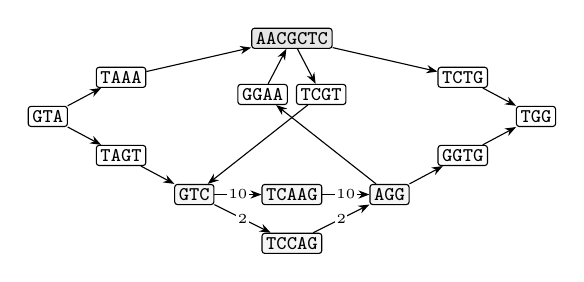
\begin{tikzpicture}[x=0.62cm,y=0.62cm,>={Stealth[length=1.4mm]},v/.style={draw,rounded corners=1pt,inner sep=1.5pt,font=\scriptsize\ttfamily}]
\node[v] (GTA) at (0,0) {GTA};
\node[v] (TAAA) at (1.5,0.8) {TAAA};
\node[v] (TAGT) at (1.5,-0.8) {TAGT};
\node[v,fill=gray!20] (AACGCTC) at (5,1.6) {AACGCTC};
\node[v] (TCGT) at (5.6,0.45) {TCGT};
\node[v] (GGAA) at (4.4,0.45) {GGAA};
\node[v,fill=gray!8] (GTC) at (3,-1.6) {GTC};
\node[v,fill=gray!8] (TCAAG) at (5,-1.6) {TCAAG};
\node[v,fill=gray!8] (TCCAG) at (5,-2.6) {TCCAG};
\node[v,fill=gray!8] (AGG) at (7,-1.6) {AGG};
\node[v] (TCTG) at (8.5,0.8) {TCTG};
\node[v] (GGTG) at (8.5,-0.8) {GGTG};
\node[v] (TGG) at (10,0) {TGG};
\draw[->] (GTA) -- (TAAA);
\draw[->] (GTA) -- (TAGT);
\draw[->] (TAAA) -- (AACGCTC);
\draw[->] (TAGT) -- (GTC);
\draw[->] (AACGCTC) -- (TCGT);
\draw[->] (AACGCTC) -- (TCTG);
\draw[->] (TCGT) -- (GTC);
\draw[->] (GTC) -- node[font=\tiny,fill=white,inner sep=0.5pt] {10} (TCAAG);
\draw[->] (GTC) -- node[font=\tiny,fill=white,inner sep=0.5pt] {2} (TCCAG);
\draw[->] (TCAAG) -- node[font=\tiny,fill=white,inner sep=0.5pt] {10} (AGG);
\draw[->] (TCCAG) -- node[font=\tiny,fill=white,inner sep=0.5pt] {2} (AGG);
\draw[->] (AGG) -- (GGAA);
\draw[->] (AGG) -- (GGTG);
\draw[->] (GGAA) -- (AACGCTC);
\draw[->] (TCTG) -- (TGG);
\draw[->] (GGTG) -- (TGG);
\end{tikzpicture}

  \caption{Twelve strings (top; spaces added for readability) and their
    de Bruijn graph for $k = 3$, uncompacted (middle; branching
    $k$-mers shaded) and compacted (bottom). \texttt{AACGCTC} is a
    unitig. \texttt{GTCAAGG} is an almost-unitig: ten strings contain
    it, and two have \texttt{GTCCAGG} instead (edge labels count the
    strings).}
  \label{fig:dbg}
\end{figure}

%MERGE: condensed from the introduction of More RLBWT Tricks
We built these \emph{shortcuts} (\Cref{sec:shortcuts}), generalised to
windows of a reference sequence, and used them to speed up
forward--backward search and BML over the RLBWTs of $T$ and $T'$. They
are beaten, however, by \emph{two-level
indexing}~\cite{BrownEtAlRLCSA,HongEtAl2024,DengEtAl2022}, which also
indexes a parse of the collection (\Cref{sec:twolevel}). Our main
contribution here (\Cref{sec:blocks}) is an encoding of the parse into
blocks of phrases that are each the lexicographically smallest
successor of the phrase before them, which lets the search cross a
whole block in one step while all three indexes stay in the same order.

\subsection{Shortcuts}
\label{sec:shortcuts}

The following observation lets a backward search notice that it has
matched a string $\beta$ from a precomputed set.

\begin{lemma}
\label{lem:detect}
If $|\beta| \le |X|$ and $\intv(X)$ is non-empty, then $\intv(X)
\subseteq \intv(\beta)$ if and only if $\beta$ is a prefix of $X$.
\end{lemma}

\begin{proof}
If $\beta$ is a prefix of $X$, every suffix starting with $X$ starts
with $\beta$. Otherwise the prefix $\beta'$ of $X$ of length $|\beta|$
differs from $\beta$, so $\intv(X) \subseteq \intv(\beta')$, which is
disjoint from $\intv(\beta)$.
\end{proof}

Let $\beta$ be the last $k$-mer of a unitig or almost-unitig $\alpha
\beta$. We store $\intv(\beta)$, the first row $f$ of $\intv(\alpha
\beta)$ and a bitvector $M$ over $\intv(\beta)$ marking the rows whose
suffixes are preceded by $\alpha$ (for a unitig, all of them, and $M$
need not be stored). When the current match $X$ has $\intv(X) =
[\mathrm{lo}, \mathrm{hi}] \subseteq \intv(\beta)$ and the pattern has
$\alpha$ immediately to the left of $X$, which we check by comparing
characters, the search jumps to
\[
\intv(\alpha X) = [f + \mathrm{rank}_1(M, \mathrm{lo}),\ f +
\mathrm{rank}_1(M, \mathrm{hi} + 1) - 1],
\]
where ranks are relative to the start of $\intv(\beta)$: by the order
preservation of LF, the marked rows of $\intv(\beta)$ are mapped in
order onto $\intv(\alpha\beta)$, and those inside $\intv(X)$ onto
$\intv(\alpha X)$. If the result is empty, the search takes ordinary
steps. Since the jump is taken only after $\alpha$ has been confirmed in
the pattern, the search returns the same result as plain backward
search, and it can also return the list of shortcuts it took. This list
is a path through the de Bruijn graph, or, with the windows below,
through a pangenome graph whose vertices are the windows, so a BWT-based
index can report the path of a match along with its interval; we find
this of more practical than theoretical interest, and do not develop
it further here.

In a pangenome, the strings that commonly precede a window are
naturally chosen from a reference $\Rref$ in the collection, such as
CHM13~\cite{NurkEtAl2022}. In the example of \Cref{fig:dbg}, with the
first string as $\Rref$ and windows of length $\ell = 4$ starting at
multiples of $4$, a search that has matched the window
\texttt{GTGG} at position $16$ can check whether the pattern has
\texttt{CAAG} to its left and, if so, cross it in one step; of the six
rows of $\intv(\texttt{GTGG})$, the one from the string with
\texttt{GTCCAGG} drops out. We stored, for each window $\beta_p = \Rref[p..p
+ \ell)$ whose interval is disjoint from those of the other windows,
shortcuts across the $2^t \ell$ characters $\Rref[p - 2^t \ell .. p)$
for $0 \le t \le \tau$ with $2^t \ell$ dividing $p$; a shortcut ends at
the start of another window, so shortcuts chain. At a window, the
search tries the longest shortcut whose string the pattern matches, and
then shorter ones.

\begin{lemma}
\label{lem:count}
Suppose $P[j - m\ell .. j + \ell) = \Rref[p - m\ell .. p + \ell)$,
the current match $P[j..|P|)$ has its interval inside that of
$\beta_p$, $P[j - m\ell .. |P|)$ occurs in $T$, and none of the windows
at $p - (m-1)\ell, \ldots, p$ was dropped because it collides with
another. Then the search reaches or passes position $j - m\ell$ of $P$
with at most $2\lceil \log_2(m+1) \rceil + \lfloor m / 2^\tau \rfloor$
shortcuts.
\end{lemma}

The proof is in \Cref{app:proofs}.

The rows of
$\intv(\beta_p)$ preceded by a longer string are a subset of those
preceded by a shorter one, so instead of one bitvector per length we
store, for each row, the number of lengths it survives, in a wavelet
tree; with $\tau = 0$ this is a single bitvector, as for an
almost-unitig. With the RLBWTs of $T$ and $T'$, and windows at the same
boundaries of $\Rref$ in both, forward and backward searches take
shortcuts in both directions.

On the chromosome~19 data of \Cref{sec:chr19-exp}, with $\ell = 25$
and $\tau = 6$, shortcuts reduce the backward steps per pattern
character from about $3.7$ to $0.45$ and make BML with $L = 1000$
$7.8$ times faster, for $1.7$ times the space of the two
RLBWTs; other values of $\ell$ and $\tau$ were slower (shorter windows
collide more often, and longer ones are crossed less often). This
speedup stays about the same as the collection grows from 16 to 64
individuals, but the space grows to $2.5$ times that of the
RLBWTs, mostly for the per-row symbols (\Cref{tab:main}).

\subsection{Two-level indexing with a syncmer parse}
\label{sec:twolevel}

Two-level indexing beats shortcuts on our data, so we describe it in
detail. Fix $k > s$. A $k$-mer over
$\{\texttt{A},\texttt{C},\texttt{G},\texttt{T}\}$ is a \emph{closed
syncmer}~\cite{Edgar2021} if its smallest $s$-mer, under an order $g$ on
$s$-mers, is its first or its last (ties included). We take $g(\gamma)$
to be a hash of the smaller of the 2-bit codes of $\gamma$ and of its
reverse $\gamma^{\mathrm{rev}}$, so $g(\gamma) =
g(\gamma^{\mathrm{rev}})$, and a $k$-mer is a closed syncmer if and only
if its reverse is. We use $k = 51$ and $s = 12$.

\begin{lemma}[Edgar~\cite{Edgar2021}]
\label{lem:window}
Among any $k - s$ consecutive $k$-mers of a string over
$\{\texttt{A},\texttt{C},\texttt{G},\texttt{T}\}$ there is a closed
syncmer.
\end{lemma}

\begin{proof}
The $k$-mers starting at positions $0, \ldots, k - s - 1$ of a string
$Y$ of length $2k - s - 1$ contain the $2k - 2s$ $s$-mers starting at
positions $0, \ldots, 2k - 2s - 1$. Let $q$ be the start of a smallest
of them. If $q \le k - s - 1$, it is the first $s$-mer of the $k$-mer
starting at $q$; otherwise it is the last $s$-mer of the $k$-mer
starting at $q + s - k \in [0, k - s - 1]$. In both cases it is
smallest in that $k$-mer.
\end{proof}

\paragraph*{The parse.}
Let $T^*$ be $T$ or $T'$. The \emph{boundaries} of $T^*$ are $b_0 = 0$ and
the starting positions of the closed syncmers in $T^*$, $b_0 < b_1 <
\cdots < b_{m-1}$. The phrases are $T^*[b_i .. b_{i+1} + k)$ for $i < m -
1$ and $T^*[b_{m-1} .. n)$, so consecutive phrases overlap by $k$
characters. We number the distinct phrases $1, \ldots, \sigma$ in the
lexicographic order of their strings, and the \emph{parse} $\Pa$ of
$T^*$ is the sequence of their ids, followed by a sentinel $0$. Within a
stretch of $T^*$ over $\{\texttt{A},\texttt{C},\texttt{G},\texttt{T}\}$,
\Cref{lem:window} bounds the length of a phrase by $2k - s$. By
the symmetry of $g$, the boundaries of $T'$ mirror those of $T$, and
the phrases of $T'$ are the reverses of those of $T$, except at the
ends; so one dictionary serves both directions.

Eddie Ferro noted that the parse at closed syncmers is
prefix-free~\cite{FerroPC}; we include a proof for completeness.

\begin{lemma}
\label{lem:order}
No phrase is a proper prefix of another, and for boundaries $b_i \ne
b_j$, $T^*[b_i .. n) < T^*[b_j .. n)$ if and only if $\Pa[i .. m] <
\Pa[j .. m]$.
\end{lemma}

\begin{proof}
A phrase contains no syncmer start strictly between its first character
and its last $k$ characters, while the last $k$-mer of every phrase
other than the last is a closed syncmer, and whether a $k$-mer is a
closed syncmer does not depend on its context. So if a phrase other than the last were a proper prefix of another
phrase, the last $k$-mer of the shorter phrase would be a syncmer
starting strictly inside the longer one;
and the last phrase ends with \$, which occurs nowhere else. Now let $h$
be the first index with $\Pa[i + h] \ne \Pa[j + h]$, which exists since
the sentinel occurs once. The phrases at $i, \ldots, i + h - 1$ and $j,
\ldots, j + h - 1$ are equal, so $T^*[b_i .. b_{i+h} + k) = T^*[b_j ..
b_{j+h} + k)$ and $b_{i+h} - b_i = b_{j+h} - b_j$. The phrases at $i +
h$ and $j + h$ are different and neither is a prefix of the other, so
they differ at some offset smaller than both lengths, and $T^*[b_i..n)$
and $T^*[b_j..n)$ compare as these two phrases do.
\end{proof}

\paragraph*{Mapping between the two levels.}
Let $B$ be the bitvector over the rows of the RLBWT of $T^*$ with $B[i] =
1$ if and only if $\mathrm{SA}[i]$ is a boundary. Every occurrence of a
closed syncmer is a boundary, so $B$ is the union of the intervals of
the distinct closed syncmers in $T^*$ plus the row of position $0$, and it
has at most that many runs of 1s; we store it run-length coded. By
\Cref{lem:order}, the $u$th 1 in $B$ (counting from $0$) is the row of
the parse with rank $u + 1$, row $0$ being that of the sentinel.

\begin{lemma}
\label{lem:bounce}
Let $q < q'$ be consecutive starts of closed syncmers in a pattern
$P[0..e)$, with $q' + k \le e$. The occurrences of $P[q..e)$ in $T^*$ are
exactly the boundaries $b_t$ such that the phrase at $t$ is $P[q .. q'
+ k)$ and $P[q'..e)$ occurs at $b_{t+1}$. Moreover, for any string $Y$
that starts with a closed syncmer, the rows of $\intv(Y)$ are all
marked in $B$, and the corresponding rows of the parse are
$[\mathrm{rank}_1(B, \mathrm{lo}) + 1, \mathrm{rank}_1(B, \mathrm{hi} +
1)]$ for $\intv(Y) = [\mathrm{lo}, \mathrm{hi}]$.
\end{lemma}

\begin{proof}
An occurrence of $P[q..e)$ at position $a$ of $T^*$ starts with a closed
syncmer, so $a$ is a boundary $b_t$. The $k$-mers of $T^*$ starting at
$a + 1, \ldots, a + q' - q$ lie inside the occurrence, so they are
closed syncmers exactly when the corresponding $k$-mers of $P$ are:
only the last is. Hence $b_{t+1} = a + q' - q$ and the phrase at $t$ is
$P[q..q' + k)$. The converse is immediate. The second claim holds
because every occurrence of $Y$ starts at a boundary, and by
\Cref{lem:order} the order of rows marked in $B$ is that of the parse.
\end{proof}

\paragraph*{Searching.}
To find the longest suffix of $P[x..e)$ that occurs in $T^*$, and its
interval, we find the starts of the closed syncmers in $P$ and look up
the ids of the phrases $P[q .. q' + k)$ between consecutive starts in a
dictionary of the phrases of $T$; the same lookup gives the id of the
reversed phrase in $T'$, so the pattern is parsed once for both
directions. The search takes backward steps on the RLBWT from $e$ to
the last syncmer start $q$ with $q + k \le e$, maps the interval to the
parse by \Cref{lem:bounce}, takes one backward step on the BWT of the
parse for each phrase of the pattern to the left, and, when a phrase is
not in the dictionary or a step on the parse fails, maps back with
select queries on $B$ and continues with backward steps on the RLBWT.

\begin{theorem}
\label{thm:twolevel}
If the dictionary lookups are correct, this search returns the same
longest suffix and interval as backward search. If $P[x..e)$ is over
$\{\texttt{A},\texttt{C},\texttt{G},\texttt{T}\}$, it takes at most $3k
- 2s - 1$ backward steps on the RLBWT, plus one step on the parse per
phrase of the pattern crossed and one that may fail.
\end{theorem}

\begin{proof}
Correctness follows from \Cref{lem:bounce} by induction over the
phrases. By \Cref{lem:window}, if $e - x \ge 2k - s - 1$ then one of the
last $k - s$ $k$-mers of $P[x..e)$ is a closed syncmer, so the search
reaches the parse after at most $2k - s - 1$ steps; otherwise it takes
at most $2k - s - 2$ steps in total. At the left end, either the search
is within $k - s - 1$ characters of $x$, by \Cref{lem:window}, or the
phrase $P[q .. q' + k)$ to the left of the current syncmer start $q'$
does not precede it in any occurrence, in which case $P[q..e)$ does not
occur by \Cref{lem:bounce} and the backward steps from $q'$ fail before
reaching $q$, after fewer than $q' - q \le k - s$ steps.
\end{proof}

Each step on the parse, like each step on the block sequence of
\Cref{sec:blocks}, is a predecessor query in one Elias--Fano list of
the runs of its BWT, grouped by symbol (\Cref{sec:prelim}); with
$r_\Pa$ runs in the BWT of the parse, it takes $O(1 + \log(\sigma m /
r_\Pa))$ time, and it touches only the runs of one symbol.

The dictionary stores the 64-bit hashes of the phrases of $T$, sorted
and split into buckets by their leading bits, with the phrases' ids in
$T$ and $T'$; it checks the whole hash, and we check at construction
time that the phrases of $T$ have distinct hashes. A phrase of the
pattern that is not a phrase of $T$ is then mistaken for one only if
its hash collides with one of $\sigma$ stored values, so if the hash
function behaves like a random function, the lookups are correct with
high probability; we have never observed an error. On our data
this dictionary takes $46$\,MiB for both directions, against
$96$\,MiB per direction for a hash table with the phrase ids, and
looking up all the phrases of the patterns, with prefetching, takes
about $1.1$ seconds, which our timings include. Splitting the patterns at runs of \texttt{N}
matters for the bound: the current parse does not split phrases at
\texttt{N}, so a phrase can be as long as a run of \texttt{N} in the
collection.

\subsection{Blocks}
\label{sec:blocks}

\paragraph*{Encodings of the parse.}
\label{sec:encodings}
%MERGE: More RLBWT Tricks' Section 5, shrunk to two sentences as agreed
After two-level indexing a search takes one step per phrase, and most
phrases of a pattern are predictable from the phrase before them, as
the characters of a unitig are. We first tried replacing each phrase by
its rank by frequency among the phrases that follow the phrase before
it~\cite{GagieHybrid2026}, but then the encoded suffixes are not in the
order of the suffixes of the parse, so the search cannot bounce between
the levels with $B$; the blocks below keep the first phrase of each
block explicit, which keeps all the indexes in the same order.

For a phrase id $x$, let $\succp(x)$ be the smallest id $y$ such that
$x y$ occurs in $\Pa$. Position $i > 0$ of $\Pa$ is a
\emph{continuation} if $\Pa[i] = \succp(\Pa[i-1])$. A \emph{block} is a
maximal substring $\Pa[a .. a + j]$ such that $a$ is not a continuation
and $a + 1, \ldots, a + j$ are; since $\succp$ is a function, the block
is determined by its \emph{symbol} $(\Pa[a], j)$, and is $\delta, \succp(\delta),
\ldots, \succp^j(\delta)$ for $\delta = \Pa[a]$. The \emph{block sequence}
$\Delta$ lists the symbols of the blocks of $\Pa$ in order, followed by
a sentinel. We order symbols by $\delta$ ascending and then by $j$
descending.

\begin{lemma}
\label{lem:blockorder}
For block starts $a \ne a'$ of $\Pa$, $\Pa[a..m] < \Pa[a'..m]$ if and
only if the suffix of $\Delta$ starting at the block of $a$ is smaller
than the one starting at the block of $a'$.
\end{lemma}

\begin{proof}
Equal symbols are equal strings of phrases followed by block starts,
so consider the first blocks that differ, $(\delta, j)$ at $a$ and $(\delta', j')$
at $a'$. If $\delta \ne \delta'$, both orders are decided by $\delta$ and $\delta'$.
Otherwise, by symmetry, let $j > j'$. The two suffixes agree on $j' + 1$
phrases, and the first continues with $\succp^{j'+1}(\delta)$. The block at
$a'$ is not the last block of $\Pa$, since the last phrase of $\Pa$
occurs only once and would then also be in the block at $a$; so the
second suffix continues with the first phrase $y$ of its next block,
which follows $\succp^{j'}(\delta)$ in $\Pa$ but is not a continuation, so $y
> \succp^{j'+1}(\delta)$ by the definition of $\succp$. So the first suffix is smaller, as its symbol is.
\end{proof}

So if $BS$ marks the rows of the parse whose suffixes start at block
starts, including the row of the sentinel, the $u$th marked row
(counting from $0$) corresponds to row $u$ of the BWT of $\Delta$, and a \emph{block step} on that BWT, with a symbol $(\delta, j)$,
prepends a whole block to the parse suffixes at block starts. We store
$\succp$, $BS$ (run-length coded when that is smaller, which on our
data it is by a factor of $9$ to $20$), the BWT of $\Delta$, the
symbols grouped by $\delta$ with their $j$'s in decreasing order, and one bit
per phrase saying whether it is a continuation anywhere in $\Pa$.

\begin{lemma}
\label{lem:space}
Let $\eta$ be the number of distinct closed syncmers in $T^*$, $\sigma$
the number of distinct phrases, $m$ the number of phrases, $r_\Pa$ and
$r_\Delta$ the numbers of runs in the BWTs of $\Pa$ and $\Delta$, $b$
the number of blocks and $s'$ the number of distinct block symbols.
Besides the RLBWT of $T^*$ and the dictionary, the parse index of $T^*$,
with blocks, takes
\[
O\bigl(\eta \log(n/\eta) + r_\Pa \log(\sigma m / r_\Pa) + r_\Delta
\log(s' b / r_\Delta) + b \log(m/b) + \sigma \log \sigma + s' \log m\bigr)
\]
bits. The dictionary, shared by $T$ and $T'$, takes $\sigma (64 - h + 2
\lceil \log_2 (\sigma + 3) \rceil) + O(\sigma)$ bits, where $2^h$, the
number of its buckets, is about $\sigma / 8$.
\end{lemma}

The proof is in \Cref{app:proofs}.

Nothing here depends on $n$ except through $\eta$, and $\eta$,
$\sigma$ and the numbers of runs grow slowly as haplotypes are added
(\Cref{sec:chr19-exp}). With 16 individuals, the parse indexes of $T$
and $T'$ take $102.5$\,MiB without blocks and $139.6$\,MiB with them,
of which the dictionary takes $46$\,MiB.

A pattern is split into blocks in the same way, using $\succp$ of the
collection. The key observation is that a block boundary in the
pattern is a block boundary in every occurrence that extends one
phrase to its left.

\begin{lemma}
\label{lem:blockstart}
If phrase $i$ of the pattern is not a continuation of phrase $i - 1$,
then in every occurrence in $\Pa$ of the pattern's phrases $i - 1, i,
\ldots$, the position of phrase $i$ is a block start.
\end{lemma}

\begin{proof}
The phrase before it in $\Pa$ is the pattern's phrase $i - 1$, and the
pattern's phrase $i$ is not $\succp$ of it.
\end{proof}

The search with block jumps proceeds as in \Cref{sec:twolevel}, except
that when the current parse interval is exact for the pattern's
phrases from $i$ on, and $i$ is a block start of the pattern whose
phrase is complete, it restricts the interval to block starts with two
rank queries on $BS$ and takes block steps, one per block of the
pattern, for as long as they succeed. In an occurrence of the pattern's
phrases from $i$ on that starts at a block start of $\Pa$, the block
boundaries of $\Pa$ are those of the pattern, since $\succp$ is a
function and by \Cref{lem:blockstart}; so, by induction, each interval
after a block step consists exactly of the occurrences of the pattern's
phrases from the current position on that start at block starts of
$\Pa$, and by \Cref{lem:blockstart} it contains every occurrence that
extends one more phrase to the left. The interval after the last block
step, however, may miss occurrences whose first phrase is a
continuation in $\Pa$. We fix this with the following rule.

\begin{lemma}
\label{lem:backup}
Suppose a sequence of $h \ge 1$ block steps ends at the pattern's
phrase $i$, the last of them crossing phrases $i, \ldots, i'$. If the
phrase $i$ of the pattern is never a continuation in $\Pa$, the parse
rows between the first and the last row of the final interval form
the exact parse interval for phrases $i, i+1, \ldots$. Otherwise,
taking parse steps for phrases $i', \ldots, i$ from the parse rows
between the first and the last row of the interval before the last
block step gives exact intervals.
\end{lemma}

\begin{proof}
In the first case, every occurrence starts at a block start, so the
final interval contains all of them, and the parse rows between its
first and last rows are all occurrences, by contiguity. In the second
case, let $J$ be the interval before the last block step, for the
pattern's phrases from $i' + 1$ on; it contains every occurrence
preceded by phrase $i'$, and the parse rows between its first and last
rows are occurrences of phrases $i' + 1, \ldots$. The rows of the true
interval outside that range are not preceded by phrase $i'$, by
\Cref{lem:blockstart}, so the parse step for $i'$ is exact, and so are
the following parse steps.
\end{proof}

After backing up, the search takes no block steps until it has crossed
phrase $i$ again. Each phrase is crossed by at most one block step and
one parse step, and each sequence of block steps ends with at most one
failed step, so \Cref{thm:twolevel} holds with at most two steps per
phrase on the parse and on $\Delta$. On our data, with 16 individuals, block jumps reduce the steps on
the parse from $23.3$ million to $3.1$ million, plus $2.5$ million block
steps, for BML with $L = 1000$.

\paragraph*{Other continuations.}
Blocks play the role of unitigs in the parse, except that a block
follows the smallest successor of each phrase rather than its only one.
The smallest successor is not the only choice that keeps the indexes in
the same order. Let $\chi$ assign each phrase $x$ one of the phrases that
follow it in $\Pa$, call position $i$ a continuation if $\Pa[i] =
\chi(\Pa[i-1])$, and give each symbol a third component, a bit saying
whether the first phrase of the next block is smaller or larger than $\chi$
of the block's last phrase. If symbols with the same $\delta$ are ordered
with the smaller ones first, by $j$ ascending, and then the larger
ones, by $j$ descending, the proof of \Cref{lem:blockorder} goes
through, and \Cref{lem:blockstart,lem:backup} do not depend on the
choice of $\chi$. With the smallest successor every bit says ``larger'', so
no bits are stored. Choosing the most frequent successor maximises the
number of continuations, and its blocks may shrink less as haplotypes
are added, since the most frequent successor of a phrase changes less
than its smallest one. We have implemented this choice and checked that
the search remains exact. On chromosome~19 with 16 individuals, it makes
blocks $3.3$ times longer, $31.4$ phrases on average instead of $9.5$,
and its blocks hardly shrink as haplotypes are added: $30.9$ phrases
with 32 individuals and $30.5$ with 64, against $8.3$ and $7.1$ with
the smallest successor. It does not yet pay off, however: a search also
takes parse steps for up to about a block at each end and when it backs
up, so with 16 individuals it takes $7.7$ million parse steps and $0.6$
million block steps for BML with $L = 1000$, instead of $3.1$ and $2.5$
million, and it is $5$ to $6\%$ slower.

\subsection{Experiments}
\label{sec:chr19-exp}

\paragraph*{Data.}
From the assemblies of release~2 of the Human Pangenome Reference
Consortium~\cite{HPRC2025,LucasEtAl2026} we took chromosome~19. The
collections consist of the reference CHM13~\cite{NurkEtAl2022}, of
$61.7$ million bases, and both haplotypes of the first 16, 32 or 64
individuals, by sample identifier, whose haplotypes each have
chromosome~19 as a single sequence of at least 90\% of the length of
CHM13; with 16 individuals there are 33 sequences and $n =
2{,}032{,}742{,}766$ characters. The patterns are haplotype~1 of the
next two such individuals, HG00423 and HG00438, of $61.7$ and $61.0$
million bases, split at runs of \texttt{N} into $4$ patterns of
$122.4$ million characters in all. All
sequences were already in the orientation of CHM13.

\paragraph*{Implementation and setup.}
The wavelet tree of our RLBWT uses rank9-style
bitvectors~\cite{Vigna2008}. We
built the RLBWTs with Big-BWT~\cite{BoucherEtAl2019}, and the parse
indexes from the collection and the RLBWTs in a streaming pass.
%MERGE: code citation moved here from the conclusions
Our code for this section is available at
\url{https://github.com/TravisGagie/MEM-finding}, in the directory \texttt{chr19}. All experiments ran
on a desktop with an Intel Core i7-8700 CPU (3.2\,GHz, 6 cores) and 16\,GiB of RAM, under Ubuntu 26.04, with
the searches pinned to one core and a single thread for every tool; we
report the median of five runs. All the methods we compare could be run
in parallel in the same way, by searching different patterns, or
different parts of a pattern, in different threads. Every configuration of ours gave the
same MEMs, with the same intervals, as plain search. For ropebwt3, which
indexes both strands and reports a MEM if it or its reverse complement
matches, we checked that all differences are reverse-strand matches:
with 16 individuals and $L = 100$, for example, ropebwt3 reports 234
MEMs that occur only on the reverse strand, and our 140 MEMs that
ropebwt3 does not report lie inside them, and with $L = 1000$ the
numbers are 5 and 2. Movi~2~\cite{ZakeriEtAl2026}, which we ran with
its regular index of both strands and a table of 10-mers, reads
\texttt{N} in the collection as \texttt{A}, and most of its differences
from our MEMs are explained in the same way, but not all: with
$L = 100$, at each size, between 140 and 281 strings reported only by
Movi~2 and 16 MEMs reported only by us remain, and with $L = 1000$ at
most 89 and 1. Many of the former are not maximal; for example, they
start a few characters after a MEM that has the same end. We have not
investigated these differences.
Ropebwt3 and Movi~2 answer a slightly more general question than our
index of $T$ and $T'$, which finds only forward-strand MEMs. Building
ropebwt3's index took $20$ and $43$ minutes with 32 and 64 individuals,
with a peak of $9.6$\,GiB.
Given the RLBWTs, building the parse indexes for both directions took
$5.4$, $7.5$ and $12.1$ minutes for 16, 32 and 64 individuals, with a
peak memory use of $1.9$, $3.5$ and $7.0$\,GiB.

\begin{table}[t]
  \centering
  \caption{Finding the MEMs of two chromosome~19 haplotypes (122.4
    million characters) with respect to collections of 16, 32 and 64
    individuals: space in MiB for both directions, and time in seconds,
    single-threaded, for BML with $L = 1000$ and $L = 100$ and for
    forward--backward (FB) with $L = 1000$. Plain search uses only the
    two RLBWTs, the shortcuts have $\ell = 25$ and $\tau = 6$, and
    ropebwt3 and Movi~2 index both strands. For Movi~2, the FB column
    gives the time to find all MEMs.}
  \label{tab:main}
  \begin{tabular}{l l r rrr}
    \toprule
    individuals & method & MiB & BML, 1000 & BML, 100 & FB, 1000 \\
    \midrule
    16 & plain search            & 314 & 290.5 & 287.3 & 287.2 \\
       & shortcuts               & 543 & 37.2 & 39.5 & 39.3 \\
       & two-level               & 417 & 12.3 & 14.5 & 13.8 \\
       & two-level, block jumps  & 454 & 8.0 & 10.3 & 9.7 \\
       & ropebwt3                & 157 & 64.3 & 65.5 & 63.1 \\
       & Movi~2                  & 554 & 25.9 & 28.9 & 57.3 \\
    \midrule
    32 & plain search            & 349 & 321.5 & 318.2 & 318.6 \\
       & shortcuts               & 699 & 40.3 & 42.2 & 41.5 \\
       & two-level               & 475 & 12.1 & 13.7 & 12.8 \\
       & two-level, block jumps  & 526 & 7.1 & 8.7 & 7.9 \\
       & ropebwt3                & 178 & 72.8 & 73.9 & 69.0 \\
       & Movi~2                  & 586 & 30.2 & 34.2 & 65.1 \\
    \midrule
    64 & plain search            & 406 & 348.7 & 345.5 & 344.3 \\
       & shortcuts               & 998 & 43.1 & 44.8 & 44.2 \\
       & two-level               & 569 & 12.9 & 14.3 & 13.4 \\
       & two-level, block jumps  & 642 & 7.1 & 8.6 & 7.7 \\
       & ropebwt3                & 212 & 79.5 & 80.2 & 76.8 \\
       & Movi~2                  & 639 & 35.5 & 40.8 & 85.1 \\
    \bottomrule
  \end{tabular}
\end{table}

\paragraph*{Results.}
\Cref{tab:main} shows the space and time of each method. With 16
individuals, the parse has $106.9$ million phrases, $4.17$ million of
them distinct, and $11.2$ million blocks, so a block has $9.5$ phrases
on average. Without shortcuts, finding the MEMs with BML and $L = 1000$
takes $3.7$ backward steps per pattern character, since a forward search
and two backward searches cover each MEM and consecutive MEMs overlap.
Two-level indexing replaces most of them by $0.19$ steps on the parse
per character, block jumps reduce these to $0.05$ steps on the parse and
on $\Delta$, and only $0.06$ backward steps per character remain on the
RLBWT. Two-level indexing with block jumps is then $36$ times faster
than plain search and $4.6$ times faster than the shortcuts, for $1.4$
times the space of the RLBWTs, less than the shortcuts take. It is $6.4$
to $8.0$ times faster than ropebwt3, whose index of both strands takes a
third of its space, and $2.8$ to $3.2$ times faster than Movi~2, whose
index of both strands, with its table of 10-mers, takes $1.2$ times its
space. With 32 and 64 individuals, it is $8.5$ to $10.3$ and $9.3$ to
$11.2$ times faster than ropebwt3, whose index takes a third of its
space, and $3.9$ to $4.3$ and $4.7$ to $5.0$ times faster than Movi~2,
whose index takes $1.1$ and $1.0$ times its space.

KeBaB~\cite{BrownEtAl2025KeBaB}, with $k = 20$, does not help here,
as it does with long reads that mostly do not match the collection: its
fragments keep more than $99.5\%$ of the characters with 16 individuals,
and more than $99.8\%$ with 32 and 64, since almost every
character of a whole chromosome lies in a long MEM, and neither plain
search, nor block jumps, nor ropebwt3 gets faster on the fragments. We
checked that the MEMs found in the fragments are exactly the MEMs of
length at least $L$.

As the collection grows from 16 to 64 individuals, the average number of
phrases per block drops from $9.5$ to $8.3$ and $7.1$: each new
haplotype adds successors to some phrases, and a phrase that used to be
the only successor of its predecessor may no longer be the smallest one.
Nevertheless, block jumps get faster: for BML with $L = 1000$ their
speedup over plain search grows from $36$ to $45$ and $49$, and over
two-level indexing without them from $1.5$ to $1.7$ and $1.8$. The
number of steps on the parse and on $\Delta$ stays at about $5$ million,
with more block steps and fewer parse steps, while plain search and
two-level indexing without jumps take more steps, presumably because the
MEMs get longer and overlap more. The space of the parse index grows
much more slowly than that of the shortcuts: from $0.44$ to $0.51$ and
$0.58$ times that of the RLBWTs, against $0.73$, $1.00$ and $1.46$.

% conclusions.tex -- owner: merging task (joint).  Section owners: request changes through NOTES.md.
\section{Conclusions}
\label{sec:conclusions}
\label{sec:conclusion}

We have described three experiments in finding MEMs with BWT-based indexes, each with a different bottleneck and a different structure that removes it.
On long noisy reads from whole genomes, the bottleneck is finding the right matches: each read's longest MEMs, found by BML with an adaptive threshold and KeBaB's filter searched longest first, avoid choosing a threshold and are both more accurate and faster than all the MEMs of a fixed length.
On short 16S reads, the bottleneck is answering each MEM: proportional credit is the most accurate split, and a complete, run-length compressed tag array, built from the BWT in space proportional to the number of runs, gives the counts it needs without locating any occurrence.
On whole chromosomes, the bottleneck is crossing long matches: two-level indexing with block jumps crosses them 28 to 49 times faster than plain backward search, still returning each MEM with its BWT interval, with structures whose space depends mostly on the distinct material in the collection.
The structure that removes one bottleneck does nothing for another: KeBaB's filter, which helps on the Zymo reads (Section~\ref{sec:zymo}), saves little on short, accurate reads or on whole chromosomes (Section~\ref{sec:chr19-exp}).

Each experiment leaves open questions.
For classification, the main one is how to make credit robust to differences between the database and the sample, including reads from taxa absent from the database, for example by correcting towards an estimated composition of the sample; we would also like to scale to GTDB.
It would be natural to bound the grammar of the tag runs in terms of $r$, $d$ and $\rho$.
We conjecture that tagging each character with the rank of its genome in a phylogenetic tree gives a differentially compressible tag array that yields counts at every rank.
For crossing long matches, the weakness we see is that blocks shrink as haplotypes are added; so far this has not hurt, but it may with larger collections.
The most frequent successor keeps blocks long (Section~\ref{sec:blocks}), but we have yet to make it pay off: that needs cheaper ends and back-ups.
The shortcuts of Section~\ref{sec:shortcuts} could also be applied directly to the parse, instead of encoding it.
We would also like to see these ideas applied to DNA alignment, where MEMs are the usual seeds~\cite{RossiEtAl2022,VarkiEtAl2025}: BML with an adaptive threshold and KeBaB's filter to find good seeds in noisy reads, tags giving reference positions~\cite{BalazEtAl2024,OO26} to answer them without locating every occurrence, and block jumps to cross the long matches of accurate reads and assemblies; we hope someone takes this up.
Finally, the three structures could be combined: block jumps with faster character-level indexes, such as Movi~2~\cite{ZakeriEtAl2026} and ropebwt3~\cite{Li2024}, and with KeBaB~\cite{BrownEtAl2025KeBaB} on noisier patterns; and tag arrays with two-level indexing, to report the taxa or the paths through a pangenome graph of long matches.


\bibliographystyle{plainurl}
\bibliography{refs}

\appendix
% app-katka-details.tex -- owner: KATKA task.
% Extracted by the merging task (2026-10-30) from tax_cpm.tex, Appendix A.  Key map and renamings applied (see NOTES.md).
\section{Experimental details}
\label{app:details}

This appendix lists what we believe is needed to reproduce our results with our implementation, KATKA, which is in the directory \texttt{katka} of \url{https://github.com/TravisGagie/MEM-finding}.
All parameters not mentioned are defaults.
On SILVA, the \emph{default configuration} finds MEMs of at least $L = 30$ bases with BML on an explicit RLCSA with a lookup table of 10-mers, and counts their occurrences with a run-length compressed tag array, for proportional credit.

\subparagraph*{Software and data.}
Cliffy's experiment scripts (\url{https://github.com/oma219/cliffy-experiments}, commit \texttt{566f647}), its read simulator MicrobeMixer (\url{https://github.com/oma219/MicrobeMixer}, \texttt{6409f5d}) with ART 2.5.8~\cite{HLMM12} and seqtk 1.4; Big-BWT (\url{https://github.com/alshai/Big-BWT}, \texttt{5b00650}); sdsl-lite (\texttt{c32874c}) with libdivsufsort.
Our own C++17 code was compiled with g++ 15.2 and \texttt{-O3 -march=native -DNDEBUG}, and the scoring scripts use Python 3.14.
The reference is SILVA 138.1 SSU Ref NR99 (\texttt{SILVA\_138.1\_SSURef\_NR99\_tax\_silva.fasta}, with \texttt{tax\_slv\_ssu\_138.1.txt} and \texttt{.tre}).
All times were measured with one thread on an Intel Core i7-8700 (3.2\,GHz, 6 cores) with 16\,GB of RAM under Linux.

\subparagraph*{Running the code.}
From that directory, \texttt{demo\_quick.sh} fetches and builds the dependencies at the commits above, downloads SILVA, builds the reference and the default index (\texttt{silva/build\_katka.sh}), and classifies 5\,000 read pairs per region that are included in the repository, with one thread and with all cores.
\texttt{demo\_full.sh} builds every index in this paper (\texttt{ALL=1 silva/build\_katka.sh}), downloads the read pairs we used (every 50th pair of our simulation, 200\,000 per region, from a release of the repository) and runs every experiment, each with its own script in \texttt{silva/}, and \texttt{pareto\_ft.py} computes the Pareto surface.
To classify reads with the default configuration and 8 threads, the command is \texttt{RZ\_COUNTS=1 rz-classify -j 8 -L 30 -l -C bac.csa -T bac.s1.tag -F 10 bac.rz reads.fq out.listings}.
With a digested index, add \texttt{-B bac.map} and use \texttt{-F 2}.
The output has Cliffy's listing format, extended with the number of occurrences in each genus, so our \texttt{rz\_score2.py}, or Cliffy's scripts without the counts, can score it.
Finally, \texttt{silva/run\_cliffy.sh} and \texttt{silva/run\_katka.sh} run Cliffy and our implementation on the same reads on one machine, first with one thread each and then with the same number of threads each, check that the parallel outputs equal the single-thread ones, and score both.

\subparagraph*{Reference text.}
We converted the FASTA to one line per sequence (\texttt{seqtk seq -U}) and ran Cliffy's \texttt{write\_silva\_genera.py} with the tree and rank files and \texttt{-n 10000}, which writes one file per genus, numbered in the left-to-right order of the SILVA tree (9\,118 files), and \texttt{doc\_to\_traversal.txt}.
As in Cliffy's pipeline, each file is reverse-complemented with \texttt{seqtk seq -r}, which also turns U into T.
We call genus $i$ document $i$.
In the text $T$ of Section~\ref{sec:index}, $G_i$ is the concatenation of the sequences of genus $i$ separated by \texttt{X}, and any character other than A, C, G, T (in either case) becomes \texttt{X}.
A text position is mapped to its document by a predecessor search over the document starts.
For Cliffy's scoring script we also need \texttt{trav\_to\_length.txt}, which gives for each genus its traversal string and the total length of its sequences.

\subparagraph*{Reads.}
For each of V1--V2, V3--V4, V4 and V4--V5 we ran the \texttt{simulate} command of MicrobeMixer's \texttt{sim\_16s\_reads.py} with the region's primer file, the SILVA FASTA and taxonomy, 10 million reads, and the aquatic abundance profile shipped with MicrobeMixer (\texttt{data/aquatic.tsv}, in which we replaced \texttt{Candidatus\_} by \texttt{Candidatus} followed by a space, to match SILVA 138.1).
This gives 10 million pairs of 250-base reads and a truth file \texttt{*\_seqtax.txt} per region.
The read files are grouped by genus, so we subsample regularly: for accuracy, pairs $0, 50, 100, \ldots$ (200\,000 pairs per region); for time, mate-1 reads $0, 5000, 10000, \ldots$ (2\,000 reads per region), which are among the former.
Each mate is classified on its own, as given (both strands are in the index).

\subparagraph*{Lookup tables.}
For each string of length $k_t$ over the alphabet (A, C, G, T, or the digest bytes) the table stores the BWT interval after searching for it, and for the sr-index also the toehold.
It is built when the classifier starts (\texttt{-F} $k_t$), in under a second.
A search for a string of length at least $k_t$ starts with a lookup of its last $k_t$ symbols.
If they do not occur, the search proceeds symbol by symbol from scratch, so that BML learns exactly where it fails.
Every configuration gives the same answers with and without a table.

\subparagraph*{Digests.}
Number A, C, G, T as 0--3 and let a $k$-mer's code be its $2k$-bit integer.
Its hash is the splitmix64 finalizer applied to the smaller of its code and its reverse complement's code.
In each maximal A/C/G/T run, every window of $w$ consecutive bases ($w - k + 1$ consecutive $k$-mers) selects \emph{all} its $k$-mers of minimum hash.
The selected $k$-mers, in text order and in their own orientation, form the digest of the run, after collapsing equal consecutive symbols.
Digests of consecutive runs are joined by \texttt{X}.
With $k = 4$ and $w = 11$, every one of the 256 codes occurs, but only 252 bytes are free (0--2 are reserved for terminators and \texttt{X} is the separator).
The rarest codes in the reference, taken in reverse-complement pairs until the rest fit (6 codes), therefore share one byte, and the others get bytes $3, 4, \ldots$ (skipping \texttt{X}) in increasing order of code.
Reverse complementing a digest reverses it and maps each byte to the byte of the reverse-complemented $k$-mer.
We digest $G_i$ and build $T$ from the digests as above.

\subparagraph*{Indexes.}
The BWT of $T$ (with one terminator) is built with Big-BWT.
The RLBWT stores the run heads in a Huffman-shaped wavelet tree and the run starts in Elias--Fano coded bitvectors (one overall and one per character).
The RLCSA stores, for each character $c$, the rows of the starts of the runs of $c$ and the cumulative lengths of those runs, either as plain 32-bit arrays or with Elias--Fano coding.
A backward step by $c$ is a predecessor search in the list of $c$, and gives the same intervals as the RLBWT.
The tag array is built without a suffix array: one pass of LF over the text gives the suffix-array samples at the BWT run boundaries, as for the r-index, and from them $\phi$ streams the suffix array from the last BWT position to the first.
Each entry is mapped to its document by a predecessor search over the document starts, and consecutive positions with the same document are merged into runs (the terminator's position gets the last document), so the memory needed is proportional to the number of BWT runs plus the number of tag runs.
The r-index~\cite{GagieNavarroPrezza2020} stores the suffix-array samples at the run boundaries and supports $\phi$ with a predecessor structure on them.
Our sr-index removes samples as in Cobas et al.~\cite{CGN21,CGN25} with parameter $s_r$, and $s_r = 0$ means no subsampling.
Reported sizes are file sizes in units of $10^9$ bytes.
A configuration's space is the sum of the structures it uses: the RLBWT or RLCSA used for backward search; the tag array (plus the RLBWT, for LF, if it is sampled and the search uses an RLCSA); the sr-index samples (plus the RLBWT, for reading run heads, if the search uses an RLCSA); and the lookup table.

\subparagraph*{BML without digests.}
Let $P[0..m)$ be a maximal A/C/G/T run of the read, skipped if $m < L$; set $x = 0$ and, while $x + L \le m$:
search backward for $P[x..x + L)$ from its right end; if the step for $P[j - 1]$ fails, set $x = j$ and repeat.
Otherwise continue backward from $x$ to the leftmost $a$ such that $P[a..x + L)$ occurs, then search forward from $a$ (backward on the reverse complement) to the largest $e$ such that $P[a..e)$ occurs.
Report the MEM $P[a..e)$ (the genera of its occurrences are those of its reverse complement's, whose interval the forward search gives), and set $x = e - L + 1$.

\subparagraph*{BML with digests.}
For a maximal A/C/G/T run $P[0..m)$ of the read with $m \ge \max(L, w)$, digest it as above, and for each window $y$ (covering bases $y..y + w - 1$) let $\mathit{lo}[y]$ and $\mathit{hi}[y]$ be the positions in the digest $\hat{P}$ of the first and last symbols it selects; both are non-decreasing in $y$.
Set $x = 0$ and, while $x + L \le m$: search backward for $\hat{P}[\mathit{lo}[x]..\mathit{hi}[x + L - w]]$; if the step for $\hat{P}[j - 1]$ fails, set $x$ to the smallest $y$ with $\mathit{lo}[y] \ge j$ (stop if there is none) and repeat.
Otherwise extend backward to the leftmost $a'$ and then forward to the largest $e'$ such that $\hat{P}[a'..e')$ occurs.
The MEM's span in the read is the interval of bases $[\mathit{left}, \mathit{right}]$, where $\mathit{left}$ is the smallest $y$ with $\mathit{lo}[y] \ge a'$, and $\mathit{right} = y_R + w - 2$ for the smallest $y_R$ with $\mathit{hi}[y_R] \ge e'$ ($\mathit{right} = m - 1$ if there is none).
Record the MEM with its span, and set $x = \max(x + 1, y_R - (L - w))$.
Finally, discard every recorded MEM whose span is contained in another's, and report the rest with their spans.

\subparagraph*{Answers and scoring.}
The listing answer for a MEM $M$ is the set $D$ of documents containing it, with the number $c_g$ of occurrences in each ($\texttt{RZ\_COUNTS=1}$).
With proportional credit, each $g \in D$ gets weight $|M| c_g / \sum_{h \in D} c_h$, and with even credit $|M|/|D|$.
With the range scheme the answer is the pair $\{g_\ell, g_r\}$ of the smallest and largest documents containing $M$, and each document from $g_\ell$ to $g_r$ gets weight $|M|/(g_r - g_\ell + 1)$.
This is Cliffy's LCA scoring (``method0'' in its scripts), since documents are in tree order.
Here $|M|$ is the length of $M$ in bases (of its span, with digests).
Weights from both mates are summed per genus (through \texttt{doc\_to\_traversal.txt}), with Cliffy's \texttt{DocProfReadSet} class handling the truth files.
A pair whose true genus is missing or ambiguous in the truth file counts as correct, as in Cliffy's script, under both of our measures.
Otherwise a pair is correct under Cliffy's rule if its true genus has the maximum weight, possibly tied, or if it has no weight at all and its true genus is not ``uncultured''.
It is \emph{strictly} correct if its true genus alone has the maximum weight.
We checked that our re-implementation of the scoring gives the same numbers as Cliffy's \texttt{classify\_silva\_readset.py} on a sample of 1\,500 pairs.

\subparagraph*{Cliffy.}
The second author built Cliffy's undigested and digested indexes with its authors' settings, and ran them and our default configuration on our 5\,000 read pairs per region, with \texttt{silva/run\_cliffy.sh} and \texttt{silva/run\_katka.sh}, on a server with two Intel Xeon E5-2407 v2 processors (8 cores in all, 2.4\,GHz) and 256\,GB of RAM.
Cliffy's two-pass construction of the undigested index writes about 2.3\,TB of temporary files (Cliffy's Table~1), more than the server's home disk holds: a first attempt failed after 40 hours, when the disk filled, having used 240\,GB of memory, and the build succeeded in 69 hours with the temporary files on a larger disk.
Classifying with it took 37\,GB of memory.
Times per read are with one thread or process, excluding loading the index (50\,s for Cliffy's undigested index), and accuracies are for Cliffy's LCA query (``method0''), scored as for our implementation.

\subparagraph*{Other classifiers.}
We ran Kraken~2~\cite{WLL19} and Tagger~\cite{DAF+25} on the same reads and the same machine as our implementation (\texttt{silva/run\_kraken2.sh} and \texttt{silva/run\_tagger.sh}).
We built Kraken~2's database with its own SILVA script (\texttt{kraken2-build --special silva}, default $k = 35$ and minimizer length 31), as Cliffy's authors did.
It downloads the same release, SILVA 138.1 SSU NR99, but indexes all of its sequences, including those not annotated down to the genus level, with SILVA's taxonomy.
Kraken~2 classifies the two mates of a pair together (\texttt{--paired}), and we scored its classifications with the part of Cliffy's script for Kraken~2, under which a pair is correct at the genus level only if Kraken~2 assigns it to its true genus.
Pairs assigned to a higher taxon, to the root or to nothing count as wrong (Cliffy's rule for pairs with no votes applies only to its own methods).
Counting also pairs assigned to an ancestor of their true genus below the domain, which that script calls vague positives, Kraken~2 reaches 84.3\%.
Tagger's authors instead built Kraken~2 with a flat hierarchy, in which a read is assigned to a genus, to the root or to nothing, so our numbers for Kraken~2 are not comparable with theirs.
For Tagger, we built an index of the same 402\,378 sequences as ours, with each sequence's genus as its tag and one strand only (Tagger handles reverse complements when classifying), and used its default parameters ($L = 25$, a 10-mer lookup table).
With $L = 30$, as for our default configuration, Tagger was no more accurate (81.05\%, 86.88\% and 92.72\% under the three rules), so we report its defaults.
Tagger assigns each read a single genus, so we classified the two mates separately and let each give its length to its genus, as we do for MEMs.
A pair whose mates are assigned different genera is then a tie, which is wrong under the strict measure, and a pair with one mate unclassified gets the other's genus.
(Tagger's authors classified single reads.)
For both tools, the times are with one thread and exclude loading the index: Kraken~2 reports its own classification time, and for Tagger we subtracted the running time of an invocation on a single read, which is dominated by loading the index.
Tagger breaks ties between genera at random, with a separate random number generator in each thread, so its outputs with one thread and with 12 differ slightly, and we scored the single-thread outputs.
If a pair's mates are assigned different genera, breaking the tie at random gives the true genus with probability 1/2 when one of them is right, so the expected accuracy is the mean of the accuracies with such pairs counted as wrong and as correct.
We measured speed separately, with \texttt{silva/run\_scale.sh}, on 200\,000 read pairs per region with 1, 6 and 12 threads, because on 5\,000 pairs a run with 12 threads takes well under a second and start-up dominates: on 5\,000 pairs, Kraken~2 was no faster with 12 threads than with one.
With 6 and 12 threads, our implementation was 5.3 and 7.7 times faster than with one, Kraken~2 4.3 and 5.2 times, and Tagger 4.5 and 5.8 times.
Our time per read in Table~\ref{tab:others}, 53.1\,$\mu$s, is its total classification time divided by the number of reads.
The 66.0\,$\mu$s elsewhere in the paper, which we use to compare our configurations, is measured differently, as the mean of per-read timings on 2\,000 reads per region, and we have not investigated the difference.
On the 5\,000 read pairs per region, the default configuration has strict accuracy 93.70\%, against 93.77\% on the 200\,000 pairs per region of Section~\ref{sec:accuracy}.

\subparagraph*{Credit schemes.}
The SILVA column of Table~\ref{tab:credit} scores one set of listings, made with \nolinkurl{RZ_COUNTS=1} and $L = 30$ for every 50th read pair, under each scheme with \nolinkurl{silva/rz_score_schemes.py}: \texttt{freq} is proportional credit, \texttt{list} is even credit, \texttt{norm} divides each count by twice the number of sequences of the genus, \texttt{one} gives the whole credit to one genus drawn with probability proportional to its count, \texttt{cliffs} gives each genus containing the MEM a uniformly random value and splits the credit evenly over the left-to-right and right-to-left maxima of these values in genus order, and \texttt{lca} spreads it over the range.
Random choices use a fixed seed.
The range row is from the rz-index run of Appendix~\ref{sec:rz}, which gives the same answers as \texttt{lca}.
The Zymo column scores the whole-read listings in the same way with \nolinkurl{tools/credit_schemes.py}, at the species level and per read, and with \nolinkurl{tools/norm_credit.py}, which divides each count by the number of reference sequences of its species, or by their total length.
In every case a read or read pair is correct only if its true taxon alone has the largest weight.

\subparagraph*{Zymo.}
We used the files that N.~Brown deposited on Zenodo (record 23251764): \nolinkurl{microbial_ref.fa.gz}, 14\,280 RefSeq sequences of seven bacterial species; \nolinkurl{microbial_reads.fa.gz}, 581\,802 ONT reads with their species from minimap2 alignments (\nolinkurl{microbial_reads.fa.class} and \nolinkurl{class.txt}); and \nolinkurl{yeast_reads.fa.gz}, 10\,245 yeast reads from the same run.
We tagged each sequence with its species, wrote one file per species, and split it into files of at most 1\,GB, keeping the sequences in their original order, so that every file is a dataset of a single species.
\texttt{rz-prep -d -s} (with \texttt{-U} for homopolymer compression) builds the text with both strands; Big-BWT builds the BWT of each dataset, single-threaded, and pfp-merge~\cite{BoucherEtAl2019} merges them; \texttt{rz-build} builds the r-index samples, \texttt{rz-tagbuild -S} the species tag array, and \texttt{rz-csabuild} the explicit RLCSA.
With homopolymer compression, $T$ has 39.28 billion characters, 73\% of the 53.74 billion without it, the BWT has 338.1 million runs (436.6 million without compression) and the tag array 448.7 million runs.
On the laptop, the largest Big-BWT run (\emph{E.~coli}, 18.2\,Gbp after compression) took 982\,s and 7.75\,GB, the merge 1\,240\,s and 7.3\,GB, the r-index samples 6\,436\,s and 6.0\,GB, and the tag array 26\,052\,s and 8.9\,GB, with the version of the construction that keeps all the runs in memory.
We classify with \nolinkurl{RZ_COUNTS=1 rz-classify -U -L 30 -D 14 -j 12}, which reads FASTA or FASTQ; $L$ and the filter's threshold apply to the compressed read, and reported spans are mapped back to the original read.
Without homopolymer compression we omit \nolinkurl{-U} in both programs and use \nolinkurl{-D 16}.
For the longest MEMs we add \nolinkurl{-X} with \nolinkurl{-L 1}, or with \nolinkurl{-L 20 -K zy.k20.kbf} for the KeBaB filter, built with \nolinkurl{rz-kbbuild} ($k = 20$, target false-positive rate 0.1) in 2\,736\,s and 0.15\,GB; \nolinkurl{tools/maxmem_roc.py} scores each read by the compressed length of its longest MEM, computed from the read, and prints the sensitivity, specificity and species accuracy for each threshold.
For SPUMONI~2's Table~2 we took the first 180, 360, 540 and 720 bases of each bacterial and yeast read: a prefix is accepted if it has at least one MEM of length at least $L$ that passes the filter, so the sensitivity is the fraction of bacterial prefixes accepted and the specificity the fraction of yeast prefixes rejected.
The species accuracy of the prefixes is with proportional credit.

\subparagraph*{Timing.}
Times are wall-clock per read, measured inside the classifier, with the index already loaded and the reads already read from disk.
They include digesting the read, finding the matches and answering them.
We report the mean over the four regions of the mean over the 2\,000 reads, all measured in a single run of \texttt{run\_pareto\_ft.sh} (with \texttt{COUNTS=1}), which also checks that every configuration gives the same answers with and without a lookup table.
For every configuration, we checked that all backends and sampling rates give identical outputs.

\subparagraph*{Parallelism and further systems optimisations.}
With \texttt{rz-classify -j}~$p$, $p$ threads share one copy of the index: each takes chunks of 256 reads from the input, and the answers are written back in input order, so the output is identical to that of a single thread (we checked this for every listing method, with and without lookup tables and digests).
The index structures are read-only during classification, and the scratch space for document listing, counting and locating, and the statistics counters, are kept per thread.
Alternatively, \texttt{silva/run\_split.sh}~$p$ splits the read file into $p$ contiguous slices, classifies them with $p$ processes and concatenates the outputs.
This needs no threads but loads $p$ copies of the index.
Beyond parallelism, we have not tuned our code at the systems level.
Backward search and LF-mapping are dominated by cache misses that depend on each other, so the natural next steps are interleaving the searches for several reads and prefetching their next memory accesses, to hide the latency of each miss behind work on other reads; huge pages, to reduce TLB misses on indexes of a few gigabytes; and memory-mapping the indexes, so that processes share them and start immediately.
Graphics processors suit data-parallel work better than pointer chasing, but they can also hide latency by running very many searches at once, so they might pay off for large batches of reads.


% app-katka-digests.tex -- owner: KATKA task.
% Extracted by the merging task (2026-10-30) from tax_cpm.tex, Appendix B.  Key map and renamings applied (see NOTES.md).
\section{Minimizer digests}
\label{sec:digest}

Like Cliffy, our implementation can index minimizer digests~\cite{RHH+04,AhmedEtAl2023} of the sequences instead of the sequences themselves.
We digest each sequence and its reverse complement as Cliffy does, with $k = 4$ and $w = 11$, but symmetrically, so that the digest of a reverse complement is the reverse complement of the digest: we use a canonical hash, select all minimizers tied for the minimum in a window, and collapse equal consecutive minimizers.
Since 4 byte values are reserved for terminators and the separator, the 256 distinct minimizers fit in a byte only once the 6 rarest share one.
The digested text has 262 million symbols and its BWT has 35.9 million runs.
To classify a read, we digest it the same way, keeping only the minimizers selected by windows lying entirely inside each match.
A window inside a match in the read is also a window inside the corresponding occurrence in the database, and selects the same minimizers there, so the digest of every DNA match occurs in the digested database.

We keep the threshold $L$ in bases rather than in digest symbols, since consecutive digest symbols can stand for very different numbers of bases.
A window of the read covers $w$ bases and selects a range of digest symbols, and these ranges move monotonically to the right as the window does.
A DNA match $P[x..x + L)$ contains exactly the windows starting in $[x, x + L - w]$, so its digest is the range of symbols they select.
BML searches backward for this range of symbols.
If the search fails at symbol $j$, then every window start $x' \geq x$ whose first window selects a symbol no later than $j$ also fails, and we jump to the first window that selects only symbols after $j$.
If the search succeeds, we extend the match to a maximal digested MEM and compute its span in bases: the longest DNA interval of the read all of whose windows select symbols within the MEM.
This finds every digested MEM whose span is at least $L$ bases and is not contained in another digested MEM's span.
We checked this against brute-force enumeration on 3\,000 reads for every $L$ from 15 to 50.
The weight of a MEM is the length of its span.

\begin{table}[t]
\centering
\caption{Classification over minimizer digests ($k = 4$, $w = 11$), with tags and proportional credit, against the default configuration and Cliffy's digested index.
All use a lookup table ($k_t = 2$ digest symbols with digestion, $k_t = 10$ bases without).}
\label{tab:digest}
\small
\begin{tabular}{lrrrrrr}
\toprule
 & space & \multicolumn{5}{c}{time per read ($\mu$s)} \\
\cmidrule{3-7}
configuration & (GB) & $L = 15$ & $L = 20$ & $L = 30$ & $L = 40$ & $L = 50$ \\
\midrule
\multicolumn{2}{l}{\emph{digests}: strict accuracy} & 92.47\% & 92.47\% & 92.48\% & 92.36\% & 92.05\% \\
\quad explicit RLCSA, tags & 0.49 & 56.6 & 54.7 & 39.3 & 32.7 & 25.2 \\
\quad Elias--Fano RLCSA, tags & 0.27 & 79.0 & 76.6 & 61.9 & 50.7 & 44.4 \\
\quad RLBWT, tags sampled with $s_r = 4$ & 0.19 & & & 220.1 & 147.0 & 114.3 \\
\addlinespace
\multicolumn{2}{l}{\emph{undigested}: strict accuracy} & 93.74\% & 93.77\% & 93.77\% & 93.48\% & \\
\quad default configuration & 1.44 & 88.6 & 79.2 & 66.0 & 57.3 & \\
\midrule
\multicolumn{7}{l}{\emph{Cliffy}~\cite{ABL25}, digests, approximate listing: 92.8--93.4\% with their scoring and reads} \\
\quad & 4.27 & \multicolumn{5}{c}{77--82} \\
\bottomrule
\end{tabular}
\end{table}

Table~\ref{tab:digest} shows that digestion makes the index three times smaller (0.49 instead of 1.44\,GB with an explicit RLCSA and tags) and classification 1.7 times faster with $L = 30$ (39.3 instead of 66.0\,$\mu$s), at a cost of 1.3 points of accuracy (92.48 instead of 93.77\%).
The digested tag array has 81.0 million runs, 2.26 times as many as the BWT, and takes 0.19\,GB (18.3 bits per run), plus 0.03\,GB for the range-minimum structure if listing.
Over digests, an Elias--Fano RLCSA is only 1.6 times slower than an explicit one, so it gives a 0.27\,GB index that is still faster than the undigested default, and sampled tag arrays on the RLBWT give the smallest indexes we built, 0.16 to 0.19\,GB.
Once the sequences are digested, building the index with an explicit RLCSA takes about 4 minutes: 132\,s for the BWT (peak memory 2.0\,GB), a few seconds for the RLCSA, and 79\,s for the tags.
Cliffy's paper reports a digested index of 4.27\,GB, almost 9 times larger, about twice as slow per read on its server, with 92.8 to 93.4\% accuracy for approximate listing with its own scoring on its own reads.
On our reads, Cliffy's LCA query on its digested index reaches 84.15\% strict accuracy (Table~\ref{tab:others}), against 92.08\% for our digested index on the same reads and server (92.48\% on 200\,000 read pairs per region).

% app-katka-alternatives.tex -- owner: KATKA task.
% Extracted by the merging task (2026-10-30) from tax_cpm.tex, Appendix C.  Key map and renamings applied (see NOTES.md).
\section{Alternatives we considered}
\label{app:alternatives}
\label{app:negative}

This appendix explains the choices behind our default configuration, by describing the alternatives we tried along the way, and some we have not tried yet.
Most of them were worse on SILVA, which consists of short, highly conserved sequences with many per genus.
Some might work better on other datasets, such as whole genomes, where the number of occurrences of matches and the compressibility of tag arrays could differ greatly.

\subsection{Which matches}
\label{app:matches}

Cliffy cuts each read into \emph{Ziv--Merhav phrases} (ZMPs), the phrases of the cross parse of Section~\ref{sec:background}: each is the longest string ending at its position that occurs in the database, and each new backward search starts at the character where the previous one failed.
The same parse underlies Relative Lempel--Ziv compression~\cite{KPZ10}, but there each phrase also stores the position of a source, which is needed to decompress.
For classification only the phrases matter, so ZMP is the more appropriate name.
Our first experiments compared ZMPs with all the MEMs of each read, found by Li's forward--backward algorithm~\cite{Li2012}, which alternates backward and forward extensions and starts each search one position after the end of the previous MEM, with the range scheme.
MEMs were more accurate than ZMPs by 0.4 to 1.3 points at the genus level (with Cliffy's scoring), both with and without digestion.
However, reads have many short MEMs, short MEMs occur many times in the database, and listing the genera containing them is expensive: with a subsampled r-index (Appendix~\ref{app:listing}), locating all the occurrences of all the MEMs of a read took 35 to 78\,ms.

Table~\ref{tab:L} shows how the threshold $L$ of BML affects accuracy with even credit.
With $L = 15$, the accuracy of the range scheme (87.3\% with Cliffy's scoring; not shown in the table, which is for even credit) is the same as with all the MEMs found by forward--backward search (87.2\%), while listing with the sr-index becomes more than 100 times faster (289\,$\mu$s per read instead of 35 to 78\,ms, with sampling parameter $s_r = 4$ and an explicit RLCSA).
Accuracy is almost unchanged up to $L = 30$, drops by about 2 points at $L = 50$ and collapses for larger $L$, as reads start to have no MEM that long.
Most of the gain in time comes from not listing the short MEMs, but BML also searches faster: forward--backward search that lists only the MEMs of length at least $L$ takes 133 to 146\,$\mu$s per read without digestion, almost independently of $L$, against 77 to 136\,$\mu$s for BML (unsampled tags, explicit RLCSA, no lookup table, $L$ from 40 down to 15), and remains slower with a lookup table (for example, 75 against 61\,$\mu$s with $L = 30$ and a 12-base table).

\begin{table}[t]
\centering
\caption{Genus-level accuracy with BML for various thresholds $L$ (mean over the four regions), listing the genera containing each MEM, with even credit.
``Strict'' counts ties and unclassified read pairs as wrong; ``theirs'' is Cliffy's scoring.
The last column is the fraction of unclassified read pairs.}
\label{tab:L}
\begin{tabular}{rccccccc}
\toprule
 & \multicolumn{3}{c}{undigested} & & \multicolumn{3}{c}{minimizer digests} \\
\cmidrule{2-4} \cmidrule{6-8}
$L$ & strict & theirs & uncl. & & strict & theirs & uncl. \\
\midrule
15 & 90.56\% & 91.59\% & 0.0\% & & 88.93\% & 89.97\% & 0.0\% \\
20 & 90.53\% & 91.68\% & 0.0\% & & 88.91\% & 89.98\% & 0.0\% \\
30 & 90.28\% & 91.83\% & 0.0\% & & 88.84\% & 90.03\% & 0.0\% \\
40 & 89.61\% & 91.93\% & 0.0\% & & 88.55\% & 90.12\% & 0.0\% \\
50 & 88.27\% & 92.01\% & 0.2\% & & 87.91\% & 90.27\% & 0.0\% \\
75 & 78.05\% & 87.46\% & 7.6\% & & 82.59\% & 89.91\% & 2.3\% \\
100 & 56.85\% & 66.13\% & 31.8\% & & 67.58\% & 77.77\% & 18.0\% \\
\bottomrule
\end{tabular}
\end{table}

The table also shows why we prefer the strict accuracy: with Cliffy's scoring, accuracy appears to \emph{increase} up to $L = 50$, but only because more read pairs end in ties among a few genera.
Even credit is also clearly more accurate than the range: with $L = 15$, by 3.5 points (strict) without digestion and by 3.6 points with it.

\subsection{How to give credit}
\label{app:freq}
\label{sec:norm}

\begin{table}[t]
\centering
\caption{Genus-level accuracy (strict / Cliffy's scoring, mean over the four regions) with even credit to each genus containing a match, credit proportional to the number of occurrences in each genus, and credit proportional to the fraction of each genus's sequences (both strands) containing the match.}
\label{tab:freq}
\begin{tabular}{lccc}
\toprule
 & even & proportional & normalised \\
\midrule
digests, $L = 15$ & 88.93 / 89.97\% & 92.47 / 92.49\% & 91.36 / 91.36\% \\
digests, $L = 30$ & 88.84 / 90.03\% & 92.48 / 92.51\% & 91.34 / 91.34\% \\
undigested, $L = 15$ & 90.56 / 91.59\% & 93.74 / 93.75\% & 92.92 / 92.92\% \\
undigested, $L = 30$ & 90.28 / 91.83\% & 93.77 / 93.79\% & 92.76 / 92.76\% \\
\bottomrule
\end{tabular}
\end{table}

Even credit, as in Cliffy's approximate listing, was our first choice, since it treats each genus containing a match alike.
Table~\ref{tab:freq} shows that proportional credit (Section~\ref{sec:accuracy}) is about 3.5 points more accurate, both with and without digestion, and that it almost eliminates ties.
Proportional credit favours genera with many sequences in SILVA, since they have more occurrences of everything.
To separate this effect from that of weighting each genus by how much of it contains the match, we also tried dividing each count $c_g$ by $2 n_g$, where $n_g$ is the number of sequences in genus $g$ and the factor 2 accounts for the two strands, so that each genus gets credit in proportion to the fraction of its sequences containing the match.
This normalised credit gains about 2.5 points of strict accuracy over even credit, but about 1 point less than proportional credit.

This does not mean that normalising is a bad idea in general.
MicrobeMixer chooses the genus of each simulated read according to the abundances in an aquatic biome, and only then a sequence of that genus, so our reads are not drawn in proportion to how well each genus is represented in SILVA.
Proportional credit then acts as a prior that a genus with many sequences in the database is more likely, and it helps only insofar as the genera that are abundant in the simulated samples are also well represented in SILVA, which is plausible.
On samples whose composition differs from that of the database, the prior could hurt, and normalising, or correcting towards a known or estimated composition of the sample, could be better.
A direct test would be to simulate reads by choosing genera uniformly, regardless of their representation in the database, and then sequences within each genus: if the advantage of proportional credit comes from the prior, it should shrink or disappear, while both kinds of weighting should still beat even credit if the rest of the gain comes from weighting each genus by how much of it contains the match.
We leave this test for future work.
On the Zymo reads, where the reference has up to 30 times as many sequences of one species as of another, normalising by the number of sequences or by their total length did not help (Section~\ref{sec:zymo-accuracy}), but almost every long MEM there occurs in a single species.

\subsection{How to list and count}
\label{app:listing}
\label{sec:sr}
\label{sec:rlcsa}

\subparagraph*{Subsampled r-indexes.}
Once we have the BWT interval of a MEM, the obvious way to find the genera containing it, and the number of occurrences in each, is to locate all its occurrences with an r-index~\cite{GagieNavarroPrezza2020} and map each to its genus.
The r-index stores two samples of the suffix array per run of the BWT.
The subsampled r-index (sr-index)~\cite{CGN21,CGN25} discards samples that are close in the text to others, so that it stores $O(\min(r, n/s_r))$ samples for a parameter $s_r$ while locating each occurrence in $O(s_r)$ time.
We first stored the BWT as an RLBWT, with the run heads in a Huffman-shaped wavelet tree and the run starts in Elias--Fano coded bitvectors.
With $s_r = 16$ and no lookup table, this index takes only 0.41\,GB and classifies a read in 477\,$\mu$s with $L = 30$.
Building it from the sequences took under 9 minutes on our desktop (347\,s for the BWT, 119\,s for the r-index samples and 43\,s to subsample them), and it is the smallest undigested index on our Pareto surface.

\subparagraph*{RLCSAs.}
Backward search on an RLBWT computes rank queries on the BWT, which become slower as the alphabet grows, and this matters especially for minimizer digests, whose alphabet has 256 symbols.
The RLCSA (Section~\ref{sec:prelim}) avoids this, and the sr-index's subsampling works the same way on an RLCSA, as in Cobas et al.'s sr-csa~\cite{CGN25}.
We still use the RLBWT's run heads to read characters when locating.
Building an RLCSA from the BWT takes a few seconds, and an explicit RLCSA makes every configuration two to four times faster than the RLBWT.

\subparagraph*{Tag arrays.}
A tag array needs no suffix-array samples, and listing or counting with it costs time proportional to the number of genera or runs in the interval, rather than to the number of occurrences, so it is much faster than locating.
It is also larger, because the tags have more runs than the BWT.
Tagger~\cite{DAF+25} stores the genus of only the last position of each BWT run, which suffices for its single-genus toehold but not for listing.
Most of the space of our tag array is in the genera of its runs, so we tried storing them for only some runs, in the spirit of subsampled r-indexes~\cite{CGN25} and of Olbrich and Ohlebusch's sampled tag arrays~\cite{OO26}.
Following Olbrich and Ohlebusch, let $e(i)$ be the run containing the LF-mapping of the first position of run $i$.
LF moves to the previous position of the text, so run $e(i)$ has the same genus as run $i$, unless the first position of run $i$ is the first position of a segment.
We store the genera of those runs, of which there are fewer than genera, since only some genus starts are the first position of a run.
The graph with edges $i \to e(i)$ has out-degree 1.
Unlike in Olbrich and Ohlebusch's setting, where tags strictly decrease along edges, it may have cycles (within a genus), so we also store the genus of one run on each cycle.
We then choose the other sampled runs greedily so that every run reaches a sampled run in fewer than $s_r$ steps.
On the digest there are 7\,467 segment boundaries and 11\,141 cycles, and we sample 24\% of the runs with $s_r = 4$ and 5\% with $s_r = 16$, which shrinks the tags from 0.19\,GB to 0.09\,GB and 0.06\,GB, respectively (without the range-minimum structure).
Sampling did not help much, and grammar-compressing the runs instead works better (Section~\ref{sec:tags}).
Computing LF needs access to the BWT, which an RLCSA does not provide, so a sampled tag array needs the RLBWT as well, which cancels most of its savings unless the RLBWT is used for backward search anyway.
Moreover, counting with sampled tags needs the genus of every run in the interval, each recovered by following LF.

\subparagraph*{The Pareto surface.}
A configuration is on the time--space--accuracy Pareto surface if no other configuration is at least as good in all three measures and better in at least one.
Table~\ref{tab:pareto} lists the configurations on this surface, out of all combinations of backend (RLBWT, Elias--Fano or explicit RLCSA), listing structure (sr-index with $s_r = 0, 4, 16$, tags with $s_r = 1, 4, 16$, or, without digestion and with $L = 30$ or 40, tags with grammar-compressed runs), lookup table ($k_t = 0, 10, 12$ bases or $0, 2$ digest symbols) and $L$ (15 to 40 bases, or to 50 with digests), all with proportional credit, so the space of a tag array does not include its range-minimum structure.
No configuration with $L < 30$ is on the surface, since $L = 30$ is at least as accurate and faster.
Without digestion, sr-indexes give the smallest configurations, run-length compressed tag arrays the fastest, and grammar-compressed runs most of those in between.
With digestion, only tag arrays appear.

\begin{table}[t]
\centering
\caption{Configurations on the time--space--accuracy Pareto surface (time per read in $\mu$s, by threshold $L$), with proportional credit.
EF stands for Elias--Fano, gramm.\ runs for tags with grammar-compressed runs (Section~\ref{sec:tags}), $s_r$ is the sampling parameter of the sr-index or of the tags, and $k_t$ is the length of the strings in the lookup table: $k_t = 2$ digest symbols with digestion and, unless stated otherwise, $k_t = 10$ bases without.
The accuracy depends only on the digestion and on $L$ (strict, mean over the four regions).}
\label{tab:pareto}
\small
\begin{tabular}{lrrrr}
\toprule
configuration & space (GB) & $L = 30$ & $L = 40$ & $L = 50$ \\
\midrule
\multicolumn{2}{l}{\emph{minimizer digests}: strict accuracy} & 92.48\% & 92.36\% & 92.05\% \\
\quad RLBWT + tags, $s_r = 16$ & 0.16 & 735.6 & 361.4 & 225.1 \\
\quad RLBWT + tags, $s_r = 4$, no table & 0.18 & 240.1 & 162.0 & 125.6 \\
\quad RLBWT + tags, $s_r = 4$ & 0.19 & 220.1 & 147.0 & 114.3 \\
\quad EF RLCSA + tags & 0.27 & 61.9 & 50.7 & 44.4 \\
\quad explicit RLCSA + tags & 0.49 & 39.3 & 32.7 & 25.2 \\
\midrule
\multicolumn{2}{l}{\emph{undigested}: strict accuracy} & 93.77\% & 93.48\% & \\
\quad RLBWT + sr-index, $s_r = 16$, no table & 0.41 & 476.9 & 389.5 & \\
\quad RLBWT + sr-index, $s_r = 16$ & 0.46 & 315.1 & 265.9 & \\
\quad RLBWT + tags, $s_r = 4$ & 0.61 & 227.8 & 197.6 & \\
\quad RLBWT + gramm.\ runs & 0.64 & 211.5 & 186.6 & \\
\quad RLBWT + tags, $s_r = 4$, $k_t = 12$ & 0.88 & 216.2 & 185.8 & \\
\quad RLBWT + gramm.\ runs, $k_t = 12$ & 0.90 & 199.1 & 177.3 & \\
\quad explicit RLCSA + sr-index, $s_r = 16$, no table & 0.98 & 193.9 & 145.3 & \\
\quad explicit RLCSA + gramm.\ runs, no table & 1.02 & 104.0 & 85.0 & \\
\quad explicit RLCSA + gramm.\ runs & 1.04 & 75.0 & 62.4 & \\
\quad explicit RLCSA + gramm.\ runs, $k_t = 12$ & 1.31 & 71.0 & 60.0 & \\
\quad explicit RLCSA + tags (default) & 1.44 & 66.0 & 57.3 & \\
\quad explicit RLCSA + tags, $k_t = 12$ & 1.71 & 62.9 & 54.4 & \\
\bottomrule
\end{tabular}
\end{table}

\subsection{Counting with rank queries}
\label{app:rank}

Instead of scanning the tag runs in a MEM's BWT interval to count its occurrences in each taxon, we could list the taxa with Muthukrishnan's algorithm and then count the occurrences of each with two rank queries on the tag array, as Sadakane's document listing allows~\cite{Sad07} and as Cobas, M\"akinen and Rossi do on a grammar-compressed document array~\cite{CMR20}.
This takes time proportional to the number of taxa containing the MEM, times the cost of a rank query, rather than to the number of tag runs in the interval.
It needs rank support on the run-length compressed tag array, for example, for each taxon, the sorted list of the starts of its tag runs with their cumulative lengths, like the lists of our RLCSA, so that a rank query is a predecessor search in one list.
It can pay off only when intervals span many tag runs of few taxa, as the intervals of short or common MEMs can on references with many genomes per taxon.
We implemented it, with explicit lists and jump tables as in our RLCSA, and compared it with scanning on the BWT intervals of the MEMs of our SILVA timing reads and of 1\% of the Zymo reads; both methods give identical counts.
On SILVA, with $L = 30$, it takes 1.32\,$\mu$s per MEM against 0.92\,$\mu$s for scanning, and its lists take 3.0\,GB against 0.97\,GB for the whole tag array: intervals with many tag runs also contain many genera, so listing alone costs almost as much as scanning.
On Zymo it wins for the rare intervals with 64 or more tag runs (1.8\,$\mu$s against up to 10\,$\mu$s), which contain many runs of few species, but these are fewer than 0.03\% of the intervals, and 99\% lie inside a single tag run, where counting is trivial; its lists take 7.3\,GB against 1.47\,GB.
On both references, counting is a small fraction of the time per read.

\subsection{LCAs without locating: the rz-index}
\label{sec:rz}

When each match votes for an LCA, we only need the leftmost and rightmost genera containing it, which are the genera of its leftmost and rightmost occurrences in the text.
The rz-index finds these without locating any other occurrence.
It combines the first KATKA~\cite{GKL22}, which found the leftmost and rightmost occurrences of a $k$-mer with range-minimum queries on grids built from LZ77 parses, with the composite indexes of Belazzougui et al.~\cite{BelazzouguiEtAl2015,BelazzouguiEtAl2017}, which pair the RLBWT with the phrase boundaries of the LZ77 parse: an occurrence that crosses or ends at a phrase boundary (a \emph{primary} occurrence) is found with a two-dimensional grid whose points are the phrase boundaries, sorted by the text that follows them and by the reversed text that precedes them, and all other occurrences are copies of primary ones.
To query the grid for a pattern, they need the BWT interval of each of its suffixes, which backward search over the RLBWT of the text provides, and the interval of the reverse of each of its prefixes, for which they keep a second RLBWT, of the reversed text.
Since our index contains both strands, we do not need that second RLBWT: we sort the phrase boundaries by the reverse complement of the text preceding them, instead of its reverse, so the intervals we need are those of the reverse complements of the prefixes, which are in the same index.
Since the leftmost occurrence of a pattern is always primary, we can also replace range reporting with range-minimum queries on the grid.
A symmetric grid built on a right-to-left parse gives the rightmost occurrence.
For the rz-index, $T$ and its reverse are parsed with a left-referencing greedy LZ77 parse in which each phrase's source starts within the previous 32\,million characters.
The two grids are built on the phrase ends of the two parses, each as a wavelet matrix with a range-minimum structure on each level, and auxiliary structures (per-level union bitvectors and scan arrays) speed up the grid queries.

Table~\ref{tab:rz} compares the rz-index with Cliffy's LCA query.
With Cliffy's own matches (ZMPs), the rz-index is 4.4 to 9 times smaller than Cliffy's index, and on our older desktop it takes 1.6 to 3 times as long per read as Cliffy reports on its server (1.6 times with the explicit RLCSA).
Its accuracy is within a few points of Cliffy's on a different set of reads: 1 point higher on V1--V2 and 1 to 4 points lower on the other three regions, which suggests that the two read sets differ somewhat in difficulty, and which served as a check on our setup.
With MEMs found by BML and $L = 50$, the digested rz-index classifies a read in 66\,$\mu$s, faster than Cliffy reports for its digested LCA query on its server, with an index 4.4 times smaller and similar accuracy.

\begin{table}[t]
\centering
\caption{LCA classification: the rz-index with ZMPs (Cliffy's matches; scored on 1 million read pairs per region) and with BML MEMs, against Cliffy's LCA query.
Accuracy is at the genus level, with Cliffy's scoring (``theirs'') and strict.
Ranges are over the four regions and single values are means, and we did not compute strict accuracy for the ZMP runs.
The rz-index sizes include auxiliary structures that speed up its grid queries.
EF stands for Elias--Fano.
Cliffy's time is for approximate listing, which uses the same index as its LCA query.}
\label{tab:rz}
\small
\resizebox{\textwidth}{!}{\begin{tabular}{llrrcc}
\toprule
 & configuration & space (GB) & time ($\mu$s/read) & theirs & strict \\
\midrule
\multirow{3}{*}{\shortstack[l]{digested\\ZMPs}} & rz, RLBWT & 0.76 & 212 & \multirow{3}{*}{83.7--87.3\%} & \\
 & rz, EF RLCSA & 0.75 & 152 & & \\
 & rz, explicit RLCSA & 0.96 & 125 & & \\
\addlinespace
\multirow{3}{*}{\shortstack[l]{undigested\\ZMPs}} & rz, RLBWT & 0.99 & 522 & \multirow{3}{*}{84.8--88.6\%} & \\
 & rz, EF RLCSA & 1.01 & 594 & & \\
 & rz, explicit RLCSA & 1.39 & 330 & & \\
\addlinespace
digested MEMs & rz, explicit RLCSA, $L = 30$ & 0.96 & 131 & 85.7\% & 85.3\% \\
 & rz, explicit RLCSA, $L = 50$ & 0.96 & 66 & 86.7\% & 84.8\% \\
undigested MEMs & rz, explicit RLCSA, $L = 30$ & 1.39 & 262 & 87.6\% & 87.0\% \\
 & rz, explicit RLCSA, $L = 50$ & 1.39 & 167 & 89.3\% & 85.5\% \\
\midrule
Cliffy LCA & minimizers & 4.27 & 77--82 & 86.3--88.5\% & \\
 & undigested & 9.01 & 199--204 & 87.5--90.2\% & \\
\bottomrule
\end{tabular}}
\end{table}

The rz-index is not on our Pareto surface, however, because with tag arrays listing costs little more than computing the LCA and is about 3.5 points more accurate with even credit, and more with proportional credit.
Computing the LCA from tags, as the smallest and largest genus listed, also gives exactly the same answers as the rz-index, about three times faster: over digests, with $L = 30$ and an explicit RLCSA, about 40\,$\mu$s per read against 131\,$\mu$s.
The rz-index may still be useful where listing is not an option, for example when the number of documents is so large that listing them is too expensive.

\subsection{Verifying digested matches}

Undigested MEMs are more accurate than digested ones, so we tried to get the best of both by verifying each occurrence of a digested MEM against the DNA and extending it to an exact match, using a Relative Lempel--Ziv representation of the database (with the longest sequence of each genus as the reference) and the positions of the minimizers.
These structures took 0.24\,GB, and verification worked, but digested MEMs are less specific than DNA MEMs (with $L = 30$, they occur in 6.0 genera on average, against 3.8), and checking their occurrences took 850\,$\mu$s per read, against 125 to 253\,$\mu$s for classifying with an undigested sr-index on an explicit RLCSA with a lookup table ($L$ from 30 down to 15).

\subsection{Combining LCAs and listing}

Listing is most expensive for MEMs with many occurrences, and for such MEMs the LCA may lose little information, so we tried answering by LCA (with the rz-index's grids) whenever a MEM has more than $K$ occurrences, or whenever its occurrences cover a fraction at least $\alpha$ of the sequences under its LCA, and listing (with the sr-index) otherwise.
With BML, few MEMs have many occurrences: the threshold $K$ saved 25 to 45\% of the time over digests, but required the grids (0.42\,GB more), and the rule based on $\alpha$ sent fewer than 1\% of the MEMs to the LCA while needing the LCA of every MEM to decide.
With tag arrays, listing is as fast as computing the LCA anyway.

\subsection{Filtering \texorpdfstring{$k$}{k}-mers instead of digesting}

KeBaB~\cite{BrownEtAl2025KeBaB} first breaks each read into \emph{pseudo-MEMs}, the maximal substrings of length at least $L$ all of whose $k$-mers pass a Bloom filter of the database's $k$-mers ($k < L$).
Every MEM of length at least $L$ lies in a pseudo-MEM, so the rest of the read can be skipped without changing the answers.
Since this keeps the accuracy of undigested matches, we asked whether it could give us the speed of digests instead.
To bound what any filter could achieve, we used exact $k$-mer membership at no cost before undigested BML (listing with tags on the explicit RLCSA).
The answers were identical, but 94 to 97\% of the bases remained in pseudo-MEMs, and the time per read dropped only from 92--99 to 72--83\,$\mu$s for $L = 30$ ($k = 20$ or $25$) and by 7 to 9\% for $L = 15$ ($k = 12$), against 42\,$\mu$s with digests and an index a third of the size (all without lookup tables).
Almost every $k$-mer of our short, accurate reads occurs in the database, and BML spends its time extending the long MEMs themselves.
KeBaB is designed for long, error-prone reads.
Brown et al.\ obtained their largest speedups by searching only each read's longest pseudo-MEMs, which risks discarding all of its long MEMs, since a long pseudo-MEM need not contain a long MEM: in their pipeline the pseudo-MEMs were chosen before any was searched.
If finding pseudo-MEMs is integrated with searching them, this risk disappears: we can search the pseudo-MEMs in decreasing order of length and stop only when we have found as many MEMs as we want that are longer than the next pseudo-MEM~\cite{BrownEtAl2025KeBaB}, or use parse indexing to bound the lengths of the MEMs that pseudo-MEMs must contain~\cite{Gagie2026pseudo}.

\subsection{Matching whole phrases}

A digest symbol names only its minimizer, not the bases up to the next one.
A one-level parse index~\cite{HongEtAl2024,BrownEtAlRLCSA,Gagie2026pseudo} instead replaces each phrase of a locally consistent parse, such as prefix-free parsing~\cite{BoucherEtAl2019} or a parse into phrases starting at minimizers, by an identifier, such as its Karp--Rabin hash, and parses the read the same way, so that matching whole phrases is exact, at about the cost of matching digests.
Only the ends of each MEM, up to about a phrase on each side, are lost.
To estimate that loss, we trimmed each MEM found with $L = 30$ by the undigested index to the part a phrase index with minimizer phrases ($k = 4$, $w = 11$) would certainly match (18.5 bases removed per MEM, on average) and listed the genera of the trimmed strings.
On 20\,000 read pairs from each of V1--V2 and V4, strict accuracy dropped by 2.3 and 3.3 points, more than digestion costs, and trimming just 2 bases from each end already cost 0.3 to 0.5 points: the ends of a MEM are where the read diverges from all but a few genera, and the middles of our MEMs occur in 219 genera on average, against 4 for the whole MEMs.
A one-level phrase index is therefore no substitute for digests on SILVA, although it might be on datasets whose matches carry less of their information at their ends.

% app-chr19.tex -- owner: More RLBWT Tricks task.
% Extracted by the merging task (2026-10-30) from paper.tex, Appendix A.  Renamings applied (see NOTES.md).
\section{Omitted proofs from Section~\ref{sec:chr19}}
\label{app:proofs}

\begin{proof}[Proof of \Cref{lem:count}]
Measure positions in units of $\ell$: the search starts at $x_0 =
p/\ell$ and must reach $a = x_0 - m$. From $x > a$, the shortcut of
length $2^t\ell$ with $t = \min(\nu(x), \tau, \lfloor \log_2(x - a)
\rfloor)$ is available, where $\nu(x)$ is the exponent of the largest
power of two dividing $x$: its string is matched by $P$, and the
resulting interval is non-empty because $P[j - m\ell .. |P|)$ occurs in
$T$. The search takes this shortcut or a longer one. A longer one
crosses more than $x - a$ windows, so it passes $a$ and is the last
shortcut needed; so it suffices to bound the number of shortcuts when
the search always takes the stated one, which leads to $x - 2^t$. While
$t = \nu(x)$ is smaller than the other two terms, subtracting
$2^{\nu(x)}$ increases $\nu$, so these shortcuts have strictly
increasing lengths, at most $2^{\lfloor \log_2 m \rfloor}\ell$: at most
$\lceil \log_2(m+1) \rceil$ of them. While $t = \tau \le \nu(x)$, each
shortcut crosses $2^\tau$ windows and keeps $\nu \ge \tau$: at most
$\lfloor m / 2^\tau \rfloor$ of them. Once $t = \lfloor \log_2(x - a)
\rfloor \le \nu(x)$, the remaining distance drops below $2^t$ while
$\nu$ stays at least $t$, so later shortcuts have strictly decreasing
lengths: at most $\lceil \log_2(m+1) \rceil$ of them. The phases occur
in this order, which gives the bound.
\end{proof}

\begin{proof}[Proof of \Cref{lem:space}]
$B$ has at most $\eta + 1$ runs of 1s, and we store their starts and the
number of 1s before each in two Elias--Fano lists, in $O(\eta
\log(n/\eta))$ bits since $m \le n$. The BWT of $\Pa$ is stored as two
Elias--Fano lists over its $r_\Pa$ runs, one of their starts offset by
symbol, in a universe of size $(\sigma + 1)(m + 1)$, and one of their
positions in the first column, in $O(r_\Pa \log(\sigma m / r_\Pa))$
bits; the BWT of $\Delta$, with $b + 1$ rows and $s' + 1$ symbols,
likewise in $O(r_\Delta \log(s' b / r_\Delta))$ bits. $BS$ marks $b + 1$
of $m + 1$ rows, in $O(b \log(m/b))$ bits as an Elias--Fano list, and we
use its run-length coding only when that is smaller. $\succp$ and the
continuation bits take $O(\sigma \log \sigma)$ bits. The symbols are
stored as an Elias--Fano list of the first symbol of each $\delta$, in
$O(\sigma + \sigma \log(s'/\sigma)) \subseteq O(\sigma + s')$ bits, and
their $j$'s, of at most $\lceil \log_2 m \rceil$ bits each. The
dictionary stores, for each phrase, the low $64 - h$ bits of its hash
and its ids in $T$ and in $T'$, which has at most $\sigma + 2$ distinct
phrases, plus the first slot of each bucket in $O(1)$ words.
\end{proof}


\end{document}
